\documentclass[12pt]{report}
\usepackage[utf8]{inputenc} 
\usepackage[T1]{fontenc} 

\usepackage{graphicx}
\usepackage{abstract}
\usepackage{mathpazo} 
\usepackage{float}
\usepackage[hyphens]{url}
\usepackage[breaklinks]{hyperref}
\usepackage{amsmath}
\usepackage[normalem]{ulem}
\usepackage{amsfonts}
\useunder{\uline}{\ul}{}
\usepackage{longtable}
\usepackage{verbatim}
\usepackage{indentfirst}
\usepackage{titlesec}

\titleformat{\chapter}[display]
  {\normalfont\bfseries}{}{0pt}{\Huge}
  
\usepackage{lipsum}

\usepackage{setspace}

\usepackage[margin=1in]{geometry}

\usepackage{adjustbox}
\usepackage{setspace}
\usepackage{amssymb}
\usepackage{mathtools}
\usepackage{graphicx}
\usepackage{subfig}
\usepackage{listings}

\begin{document}


\newtheorem{thm}{Theorem}[section] 
\newtheorem{defn}[thm]{Definition} 
\newtheorem{ex}[thm]{Example}
\newtheorem{pro}[thm] {Proof}
\newtheorem{cor}[thm] {Corollary}
\newtheorem{lem}[thm] {Lemma}
\newtheorem{rmk}[thm] {Remark} 
\newtheorem{prop} [thm] {Proposition}

% Title Page ------------------------------------------
\begin{titlepage} 
	\newcommand{\HRule}{\rule{\linewidth}{0.5mm}} 
	\center 
	
	\textsc{\LARGE Wilfrid Laurier University}\\[1.5cm] % School name
	
	\textsc{\Large ST 562 - Regression Analysis}\\[0.5cm] % Course name
	
	\textsc{\large Department of Mathematics}\\[0.5cm] % Department name
	
	\HRule\\[0.4cm]
	{\huge\bfseries Factors Influencing Highway Crash Rates}\\[0.4cm] % Document name
	
	\HRule\\[1.5cm]
	\begin{minipage}{0.4\textwidth}
		\begin{flushleft}
			\large
			\textit{Author}\\
			Austin Sammon % Your name
		\end{flushleft}
	\end{minipage}
	~
	\begin{minipage}{0.4\textwidth}
		\begin{flushright}
			\large
			\textit{Instructor}\\
			Dr. Zilin Wang % Instructor
		\end{flushright}
	\end{minipage}
	\vfill\vfill\vfill
	
	{\large Tuesday December 20, 2022} % Date
	
	\vfill\vfill\vfill
	
\includegraphics[width=0.2\textwidth]{Wlu_colour_logo.jpg}\\[0.1cm] 
	
	\vfill
	
\end{titlepage}

% End of Title Page ------------------------------------

\renewcommand{\abstractname}{Abstract}
\renewcommand{\abstractnamefont}{\normalfont\Huge\bfseries}

\doublespacing
\begin{abstract}

Highway collisions are one of the leading causes of serious injuries and deaths, causing considerable financial hardship and social consequences. This project aims to identify factors that are significantly associated with highway accident rates. After completion of a diagnostic check and adequacy test on the original data and model, subset selection was conducted and the optimal fitted model was found to be $\hat{y} = 10.1711 - 0.09848x_{3} + 0.09476x_{5} - 0.12877x_{6} - 0.05988x_{8}$. This final model possessed an $R_{j}^2$ value of 0.6835 indicating the model is able to explain a majority of the variance. The hypothesis tests on the model found that the fitted regression model is significant, and only the truck volume was deemed not relevant in predicting the collision rate on highways. We see that the number of access points demonstrates a positive effect, while the length of the highway and speed limit demonstrate negative effects on the rate. Through the use of this model, governments can optimize the design and construction of new highways to reduce crash rates.
\end{abstract}

\tableofcontents

\doublespacing
\chapter{Introduction}
As society advances, road transportation becomes increasingly necessary and popular. As such an economy's growth and social progress are largely dependent on its road transport systems. A vital aspect of these transport systems is the presence of highways. These highways serve to facilitate medium and long distance travel for a large volume of traffic, connecting distant cities within a province or country. Highways differ from general inner-city roads in the fact that they have higher speed limits, traffic barriers or guardrails, and do not permit pedestrians, non-motorized vehicles, or slow vehicles to access them. In line with the increase in highway usage, the frequency at which highway accidents occur also increases.

Highway collisions are one of the leading causes of serious injuries and deaths, causing considerable financial hardship and social consequences. Based on data from the Ontario Ministry of Transportation, highway accidents are the $6^{th}$ leading cause of death among Canadians, and the total social costs for all highway accidents alone amounted to 18 billion dollars in 2004 \cite{Gov}. It is common for highway accidents to cause bottlenecks and blockades, which can lead to further collisions occurring. Achieving safety and efficiency on highways is dependent on the prevention and reduction of motor vehicle collisions. In order to prevent these types of accidents, this study sought to identify factors that are significantly associated with the frequency of such events.

The data being used to help identify potential factors influencing collision frequency is taken from the data set \textit{Highway1} \cite{Data}. This data set originated from an unpublished research paper written by Carl Hoffstedt. It includes data on accident rates on highways per million vehicle miles, as well as other highway metrics such as truck volume, average daily traffic count, and speed limits. The use of and manipulation of this collected highway data will enable us to determine whether there is a correlation between accident rates and the various parameters taken into consideration during highway construction. By doing so, future highways can be made safer for everyone. 

To determine the impact of the alterable variables a linear regression model will be fit to the data. Hypothesis tests will be conducted on the model to determine the statistical significance of certain variables as well as the model in general. From there a diagnostic check and adequacy test will be conducted on the model to verify preliminary assumptions and check for presence of multicollinearity, high leverage points, influential points, and outlier points. Once all of these potential problems have been addressed the final linear model will be compared to a non parametric model. Note the decisions made in this study are based on a $95\%$ confidence level.

The methodology used to analyze the data in this study will be described in greater detail in section 2 of this report. Section 3 will outline the data analysis, including any preliminary observations that were made, an adequacy evaluation of the model, and any inferences that could be drawn from the hypothesis tests. Any and all conclusions drawn from the analysis, as well as any weaknesses in the model, will be presented in the final section of this report.

\chapter{Methodology}
\section{Building a Linear Regression Model}

To construct a regression model for the data several options will be constructed and compared to determine which best fits the spread of the data. The first model we look at is a multiple linear regression model, which takes the general for of 
\begin{equation}
    y = \beta_{0} + \beta_{1}{x_{1}} + \beta_{2}{x_{2}} + ... + \beta_{k}{x_{k}} + \varepsilon
\end{equation}

Where y is the response variable, $x_{1} ... x_{k}$ are the regressor variables, $\beta_{0} ... \beta_{k}$ are the unknown parameters or regression coefficients that relate the x's to y, and the $\varepsilon$ is the error term associated with the model. This can equivalently be written in matrix form as $y = {X}\underset{\sim}\beta + \underset{\sim}\varepsilon$ with 
\begin{equation*}
\underset{\sim}y = 
    \begin{bmatrix}
    y_{1} \\
    y_{2} \\
    \vdots \\
    y_{n}
    \end{bmatrix}
X = 
    \begin{bmatrix}
    1 & x_{11} & x_{12} & \dots & x_{1k}\\
    1 & x_{21} & x_{22} & \dots & x_{2k}\\
    \vdots & \vdots & \vdots & \ddots & \vdots \\
    1 & x_{n1} & x_{n2} & \dots & x_{nk}
    \end{bmatrix}
\underset{\sim}\beta = 
    \begin{bmatrix}
    \beta_{0} \\
    \beta_{1} \\
    \vdots \\
    \beta_{k}
    \end{bmatrix}
\underset{\sim}\varepsilon = 
    \begin{bmatrix}
    \varepsilon_{1} \\
    \varepsilon_{2} \\
    \vdots \\
    \varepsilon_{n}
    \end{bmatrix}
\end{equation*}

Because the parameters $\beta_{0} ... \beta_{k}$ are unknown they must be estimated, this is done via least squares estimation. In using this method it is assumed that the error term $\varepsilon$ in the model has E($\varepsilon$) = 0, Var($\varepsilon$) = $\sigma^2$, and that the errors are uncorrelated. Before beginning the derivation several key identities are shown below, with $\underset{\sim}z$ a p $\times$ 1 column vector, $\underset{\sim}a$ a 1 $\times$ p row vector, and A a p $\times$ p matrix.
\begin{equation*}
\begin{split}
    \underset{\sim}z = \underset{\sim}a^{T}y \longrightarrow \frac{\partial \underset{\sim}z}{\partial y} = \underset{\sim}a\phantom{i}
    \\
    \underset{\sim}z = y^{T}y \longrightarrow \frac{\partial \underset{\sim}z}{\partial y} = 2y
    \\
    \underset{\sim}z = \underset{\sim}a^{T}Ay \longrightarrow \frac{\partial \underset{\sim}z}{\partial y} = A^{T}\underset{\sim}a
    \\
    \underset{\sim}z = y^{T}Ay \longrightarrow \frac{\partial \underset{\sim}z}{\partial y} = 2Ay\phantom{i}
\end{split}
\end{equation*}
The first step is to minimize the sum of squares of the errors with respect to $\underset{\sim}\beta$.

\begin{equation}
    S(\underset{\sim}\beta) = \sum_{i=1}^n \varepsilon_{i}^2
    = \underset{\sim}\varepsilon^T \underset{\sim}\varepsilon
    = (\underset{\sim}y - {X}\underset{\sim}\beta)^T(\underset{\sim}y - {X}\underset{\sim}\beta)
\end{equation}
Expanding the end expression results in
\begin{equation}
    S(\underset{\sim}\beta) = \underset{\sim}y^{T}\underset{\sim}y - {2\underset{\sim}y^{T}X}\underset{\sim}\beta + \underset{\sim}\beta^{T}X^{T}X\underset{\sim}\beta
\end{equation}
Now differentiating with respect to $\underset{\sim}\beta$ and setting equal to 0 we obtain
\begin{equation}
    \left. \frac{\partial S}{\partial \underset{\sim}\beta}\right|_{\hat{\underset{\sim}\beta}} = -2X^{T}\underset{\sim}y + 2X^{T}X\hat{\underset{\sim}\beta} = 0
\end{equation}
\begin{equation*}
\begin{split}
    X^{T}X\hat{\underset{\sim}\beta} = X^{T}\underset{\sim}y
    \\
    \hat{\underset{\sim}\beta} = (X^{T}X)^{-1}X^{T}\underset{\sim}y
\end{split}
\end{equation*}
$\hat{\underset{\sim}\beta}$ is considered the best linear unbiased estimator of $\underset{\sim}\beta$. To obtain the fitted model $\hat{\underset{\sim}y} = X\hat{\underset{\sim}\beta}$ we simply substitute in the least squares estimator for $\hat{\underset{\sim}\beta}$ to get $\hat{\underset{\sim}y} = X(X^{T}X)^{-1}X^{T}y = Hy$. Where $H = X(X^{T}X)^{-1}X^{T}$ is referred to as the hat matrix mapping the vector of observed values into a vector of fitted values.

\section{Estimation of Error Variance}

The error variance $\sigma^2$ is required for many of the statistical methods that can be applied to the model. To estimate it we require the residual values which are the differences between the observed value $y_{i}$ and the corresponding fitted value $\hat{y_{i}}$ for i = 1...n that is 
\begin{equation}
    \underset{\sim}e = \underset{\sim}y - \hat{\underset{\sim}y} = \underset{\sim}y - X\hat{\underset{\sim}\beta} = (I - H)\underset{\sim}y
\end{equation}
Now to estimate $\sigma^2$ we use the following relation where $\sum_{i=1}^n e_{i}^2$ is the sum of squared residuals for the model.
\begin{equation}
    \sigma^2 = \frac{1}{n-k-1} \sum_{i=1}^n e_{i}^2
\end{equation}

\section{Constructing a Hypothesis Test}
To determine if there is a linear association between Y and any of $x_{1} ... x_{k}$ hypothesis tests on individual regressor coefficients as well as on the entire model are conducted. 

When performing hypothesis tests on individual parameters the null hypothesis is of the form $H_{0}: \beta_{k} = a$ with the alternative being $H_{1}: \beta_{k} \neq a$, when testing for a linear association a is set equal to 0. The observed test statistic ($t_{0}$) used to determine the outcome of the test is then calculated using the following equation where $c_{jj}$ is the $(j+1)^{th}$ diagonal entry in the $(X^{T}X)^{-1}$ matrix.
\begin{equation}
    t_{0} = \frac{\beta_{j} - a}{\sqrt{\sigma^{2}c_{jj}}} \sim t_{n-k-1}
\end{equation}

When the calculated test statistic is compared with the associated critical value, \\$|t_{0}| > t_{\alpha/2, n-k-1}$ is considered the rejection region. Where $t_{\alpha/2, n-k-1}$ is the critical value taken from the t-distribution table for a specific significance level $\alpha$ and degrees of freedom. The p-value associated with the observed test statistic can also be used to determine whether to reject the proposed hypothesis or not, its rejection region is when the \\ p-value < $\alpha$, and can be calculated using equation $\eqref{pval}$.
\begin{equation} \label{pval}
    \text{p-value } = 2(1 - P(T \leq |t_{0}|))
\end{equation}

To construct a test to determine the significance of the regression model as a whole the null hypothesis is of the form $H_{0}: \beta_{1} = \beta_{2} = ... = \beta_{k} = 0$ with the alternative being $H_{1}:$ at least one $\beta_{j} \neq 0$. In order to calculate the observed test statistic ($F_{0}$) used to determine the test outcome, the following values must be calculated as follows $\eqref{SSMS}$. The analysis of variance (ANOVA) table, table ($\ref{tab:GA}$) is a compilation of all data needed to calculate $F_{0}$.  

\begin{equation} \label{SSMS}
   \begin{split}
       SS_{Reg} = \sum_{i=1}^n ({y_{i} - \bar{y_{i}}})^2 \phantom{332}
       SS_{Res} = \sum_{i=1}^n (y_{i} - \hat{y_{i}})^2 \phantom{323}
       SS_{T} = SS_{Reg} + SS_{Res}
       \\
       MS_{Reg} = \frac{SS_{Reg}}{n} \phantom{332}
       MS_{Res} = \frac{SS_{Res}}{n - k - 1} \phantom{3323333333333}
   \end{split} 
\end{equation}
\begin{table}[H] 
\caption{General ANOVA Table} \label{tab:GA}
\medskip
\centering
\begin{tabular}{ccccc}
\textbf{Source} & \textbf{Sum of Squares} & \textbf{Degree of Freedom} & \textbf{Mean Squares} & \textbf{$F_0$} \\ \hline\\
Regressors      & $SS_{Reg}$              & n                          & $MS_{Reg}$            & $MS_{Reg} / MS_{Res}$  \\\\
Residuals       & $SS_{Res}$              & n - k - 1                  & $MS_{Res}$            &               \\\\
Total           & $SS_{T}$                & n - 1                      &                          &              
\end{tabular}
\end{table}

In comparing the calculated test statistic $F_0$ with the associated critical value $F_{\alpha,k,n - k - 1}$, $F_{0} > F_{\alpha,k,n-k-1}$ is considered the rejection region. $F_{\alpha,k,n - k - 1}$ is the critical value taken from the F-distribution table for a specific significance level $\alpha$ and degrees of freedom. As with the F-statistic, the corresponding p-value can be used to decide whether the hypothesis should be rejected, its rejection region is the same as prior, if the p-value < $\alpha$.

\section{Testing for Multicollinearity} 
In this paper there are three methods used to determine if the model showed signs of multicollinearity, a check to see if the p-values for the individual coefficients matched up with the test on the full model, the plot of the correlation matrix, and the variance inflation factors. A more robust description of the last 2 methods is given below, the first method is excluded as the description in the Data Analysis section is sufficient.

The correlation matrix of the model is can be represented by the matrix $\rho$ in figure ($\ref{fig:Cov}$), where the $r_{ij}$ are the off diaginal elements of the matrix $X^{T}X$. Values close to 1 and -1 indicate that regressors $x_i$ and $x_j$ are nearly linearly dependent. 

\begin{equation}
\rho = 
    \begin{bmatrix} \label{fig:Cov}
    1      & r_{12}     & r_{13} & \dots  & r_{1k}\\
    r_{12} & 1          & r_{23} & \dots  & r_{2k}\\
    r_{13} & r_{23}     & 1      & \dots  & r_{3k}\\
    \vdots & \vdots     & \vdots & \ddots & \vdots \\
    r_{1k} & r_{2k}     & r_{3k} & \dots  & 1
\end{bmatrix}
\end{equation}

To calculate the variance inflation factors (VIFs) for the model the relation in equation $\eqref{VIF}$ is used. Where $R_{j}^2$ is the adjusted $R^2$ value for the model defined as below. Alternatively the main diagonal elements of the inverse of $\rho$ can also be used to calculate the variance inflation factors. Any two regressors $x_i$ and $x_j$ that are highly correlated will have a large $R_{j}^2$ value and as a result high $VIF_j$. We identify any $VIF_j \geq 10$ as an indicator of multicollinearity.

\begin{equation} \label{VIF}
    VIF_{j} = \frac{1}{1 - R_{j}^2} \phantom{333} 
    R_{j}^2 = 1 - \frac{{SSE}/{n - k - 1}}{{SST}/{n - 1}}
\end{equation}

\section{Diagnostics for Leverage and Influence}
When dealing with influential points in a dataset there is again three methods we use that lead to the identification of influential points. The first method applied to the data is a test for outliers, which focuses on the residuals specifically observations with large residuals. The residuals (e) can be calculated using $\eqref{Res}$, when dealing with a sufficiently large n or sample size it is best to standardize the residuals ($r_{i}$) to normal (0,1) before trying to identify any outliers. To standardized the residuals you simply just divid the individual residual by the standard error times the root of one minus its corresponding diagonal element in the hat matrix $\eqref{StdRes}$. To determine which observations are outliers we look for points that possess standardized residuals > 3.

\begin{equation} \label{Res}
    e = y - \hat{y} = Iy - Hy = (I - H) y
\end{equation}

\begin{equation} \label{StdRes}
    r_i = \frac{e_i}{s_e\sqrt{1 - h_i}} \phantom{3} {\sim} \phantom{3} N(\mu = 0, \sigma^ 2 = 1)
\end{equation}

The next test conducted on the data is a test for high leverage points, which makes use of the hat matrix to identify this type of influential observations. Given that $Var(\hat{y}) = \sigma^{2}H$ and $Var(e) = \sigma^{2}(I-H)$ we can say that the hat matrix determines the variances and covariances of $\hat{y}$ and e. So essentially, we can interpret each element $h_{ij}$ of the matrix H as an amount of leverage exerted by the $i^{th}$ observation $y_{i}$ on the $j^{th}$ fitted value $\hat{y}_{j}$. More specifically we will focus on the diagonal elements $h_{ii}$, and consider any observation whose hat diagonal is greater than twice the average $\frac{2p}{n}$ sufficiently differs from the rest of the data to be taken as a leverage point. Where $p = k+1$ and k denotes the number of regressor variables.

\begin{equation} \label{HLev}
    h_{ii} = \underset{\sim}{x^{T}_{i}}(X^{T}X)^{-1}\underset{\sim}{x_{i}} > \frac{2p}{n} = \frac{2(k+1)}{n}
\end{equation}

The most common test for influential points is a measure of the cook's distance ($D_{i}$). The cook's distance is a measure of the squared distance between the least squares estimate based on all n points $\hat{\underset{\sim}\beta}$ and the estimate obtained by deleting the $i^{th}$ point, $\hat{\underset{\sim}{\beta_{i}}}$. The general equation for calculating the cook's distance is given by $\eqref{CDGen}$ but can be rewritten as $\eqref{CDSim}$. A measure of $D_{i}$'s magnitude is usually determined by comparing it to $F_{\alpha,p,n-p}$, but since $F_{\alpha,p,n-p} \simeq 1$ we take any points with $D_{i} > 1$ to be influential points.

\begin{equation} \label{CDGen}
    D_i = \frac{(\hat{\underset{\sim}{\beta_{i}}} - \hat{\underset{\sim}\beta})^{T}X^{T}X(\hat{\underset{\sim}{\beta_{i}}} - \hat{\underset{\sim}\beta})}{pMS_{Res}}
\end{equation}

\begin{equation} \label{CDSim}
    D_i = \frac{1}{p}r_i^2\frac{h_i}{1-{h_i}}
\end{equation}

\section{Adequacy Check}
\subsection{Breusch-Pagan Test}
The Breusch-Pagan Test is a test used to determine if heteroscedasticity or non constant error variance is present in a model. When performing tests of this nature the null hypothesis is of the form $H_{0}:$ homoscedasticity is present with the alternative being $H_{1}:$ heteroscedasticity is present. The observed test statistic labelled "BP" is used to determine the outcome of the test. To calculate it a new regression model is constructed with the original data as the predictors and $g_{n} =\frac{e_{n}^2}{\hat{\sigma}^2}$ as the response variable, where $e_{n}^2$ is the $n^{th}$ residual. Then calculating the explained sum of squares $\sum_{i=1}^n g_{n}\hat{g}_{n}$ = $\underset{\sim}{g}^T\hat{\underset{\sim}{g}}$ leading to the test statistic being of the form
\begin{equation}
    BP = \frac{1}{2}(\underset{\sim}{g}^TX(X^{T}X)^{-1}X^{T}\underset{\sim}g)
\end{equation}

When the calculated test statistic is compared with the associated critical value, \\$BP > \chi^{2}_{\alpha,n-k-1}$ is considered the rejection region. Where $\chi^{2}_{\alpha,n-k-1}$ is the critical value taken from the chi-square distribution table for a specific significance level $\alpha$ and degrees of freedom. The p-value associated with the observed test statistic can also be used to determine whether to reject the proposed hypothesis or not, its rejection region is when the p-value < $\alpha$.

\subsection{Box-Cox Transformation}
When non constant error variance or non-normality is identified in a model one of the methods to correct it is to apply a Box-Cox transformation. This type of transformation is called a power transformation where the response variable is transformed via g(y) = $y^{\lambda}$ with the restriction of strictly positive response variables. Taking the form
\begin{equation}
    g_\lambda(y) = \left\{
        \begin{array}{lr}\displaystyle\frac{y^\lambda - 1}{\lambda} &  \lambda \neq 0\\
        & \\
       \dot{y}\log(y) &  \lambda = 0
     \end{array}
   \right.
\end{equation}
Where $\dot{y} = ln^{-1}(\frac{1}{n}\sum_{i=1}^n ln(y_{i}))$ is the geometric mean of the observations and $\lambda$ is chosen by maximizing the log-likelihood,
\begin{equation}
    L(\lambda) = -\frac{n}{2}\log(\frac{\text{SS}_{res \lambda}}{n}) + (\lambda -1)\sum \log(y_i)
\end{equation}
A $100(1 - \alpha)\%$ confidence interval for $\lambda$ is,

\begin{equation}
    \left\{ \lambda :  L(\lambda) > L(\hat{\lambda}) - \frac{1}{2}\chi_{1,\alpha}^2  \right\}
\end{equation}
which can be plotted and allows for us to quickly select an appropriate $\lambda$ for the transformation.

\subsection{Weighted Least Squares}
In the event that the errors are uncorrelated but have non constant variance weighted least squares regression can be implemented to attempt to deal with the heteroscedasticity. Weighted least squares places weights on the observations such that observations with small error variances are given more weight since they contain more information than those with large error variances. This method assumes the error term $\varepsilon \sim N(0,\sigma^{2}V)$ with 
\begin{equation}
V = 
    \begin{bmatrix}
    \frac{1}{w_1}      & 0     & \cdots & 0\\
    0 & \frac{1}{w_2}          & \cdots & 0\\
    \vdots & \vdots     & \ddots      & \vdots\\
    0 & 0     & \cdots & \frac{1}{w_n}
\end{bmatrix}
\end{equation}
We then let $W = V^{-1}$, with W a diagonal matrix, with diagonal elements or weights $w_{1}, w_{2}, . . . , w_{n}$. Applying the weightings to the normal least squares estimation leads to the estimator

\begin{equation}
    \hat{\underset{\sim}\beta} = (X^{T}WX)^{-1}X^{T}W\underset{\sim}y
\end{equation}
Where $\varepsilon \sim N(0,\sigma^{2})$ and weighted least squares estimate of $\beta$ is still the best linear unbiased estimator.

\subsection{Durbin-Watson Test}
The Durbin-Watson Test is a test that determines if there is correlation between residuals in a model. The null hypothesis of this test is of the form $H_{0}:$ Correlation of the error is zero with the alternative being $H_{1}:$ Correlation of the error non-zero. The observed test statistic labelled "DW" is used to determine the outcome of the test and calculated using the following equation.
\begin{equation}
    DW = \frac{\sum_{i=2}^n (e_{i} - e_{i-1})^2}{\sum_{i=1}^n e_{i}^2}
\end{equation}

The calculated test statistic is compared with the observed test statistic from the Durbin-Watson table to draw a conclusion on the test. Alternatively the calculated test statistic can be compared to 2, and if DW $\approx$ 2, the residuals may not be correlated but if DW isn't close to 2, the residuals may by correlated.

\section{Variable Selection}
In this study, the exhaustive method of variable selection is used due to the relatively few predictors, so this will be the only approach discussed. This method compares all $2^p$ possible combinations of regressor variables for model construction to determine the best model for the data and which predictors should be included. Each model is compared using specified criteria to determine which should be used going forward, in this study two criteria are used to rank the models, the first being the $R_{j}^2$ value. Where the model with the largest $R_{j}^2$ value is the most preferred model. The second being the Mallow's $C_{p}$ value, which is estimated following the equation below.
\begin{equation}
    \hat{\Gamma}_{p} = \frac{SS_{Res}}{\hat{\sigma}^2} - n + 2p
\end{equation}
Where p = k + 1 and the most preferred subset of variables corresponds to the model with $\hat{\Gamma}_{p}$ closest to p.

\section{Non-parametric Regression}
Non-parametric regression is based on developing a model-free basis for predicting the response to a data set and is closely related to local polynomial regression. It uses the data from a neighborhood around a specified location of interest to estimate the response. It follows a similar starting point as in polynomial regression with

\begin{equation}
    E[Y|\underset{\sim}{x}] = m(\underset{\sim}{x})
    \label{nonparam}
\end{equation}
But in this case with m(..) being unknown. We will estimate $m(x)$ locally to determine the overall shape of the regression line. This is done using the Taylor polynomial where 
\begin{equation}
    \small{m(x) \approx m(x_0) - (x-x_{0})m'(x_0)+ \frac{1}{2}(x-x_{0})^{2}m"(x_0) +\cdots+\frac{(-1)^q}{q!}(x-x_0)^qm^{(q)}(x_0)}
\end{equation}

Since each observation of x will contribute differently to the estimation of $m(\underset{\sim}{x_{0}})$ a weight is applied to each of the x's. This weighting is given by,
\begin{equation}
    W_{i0} = k(\frac{x_{i}-x_0}{h})
\end{equation}
Where $h$ is the bandwidth or the toning parameter of the neighbourhood and $k$ as the weight proportional to the distance between $x$ and $x_0$. Giving the weightings matrix 
\begin{equation}
W = 
    \begin{bmatrix}
    W_1      & 0     & \cdots & 0\\
    0 & W_2          & \cdots & 0\\
    \vdots & \vdots     & \ddots      & \vdots\\
    0 & 0     & \cdots & W_n
\end{bmatrix}_{n\times n}
\end{equation}
In comparing the local polynomial regression model $\eqref{locploy}$ to the non-parametric equation we see that the local polynomial can provide a set of estimates for $m(\underset{\sim}x)$. 
\begin{equation} \label{locploy}
    y = \gamma_0+\gamma_1(x-x_0)+\cdots+\gamma_q(x-x_0)^q+\varepsilon
\end{equation}
Similar to a parametric equation, we can construct the least square estimate for the non-parametric equation
\begin{equation}
        \underset{\sim}{\gamma} = (X^TWX)^{-1}X^TW\underset{\sim}{y}
\end{equation}
Where, $\hat{\gamma}_0 = \hat{m}(x_0), \hat{\gamma}_1 = \hat{m'}(x_0), ...   , \hat{\gamma}_q = \hat{m^{q}}(x_0)$

\chapter{Data Analysis}
\section{Preliminary Remarks}
As mentioned prior the data being used to in this study is historical data taken from the data set \textit{Highway1} \cite{Data}. It should be noted that this dataset contains data from 39 sections of large highways within the state of Minnesota and was collected in 1973. The explanatory variables examined in this study are traffic volume, number of lanes, speed limit, length of highway, lane width, number of access points, truck volume, and shoulder width. To begin the data analysis, plots of each explanatory variable versus the response variable were constructed and can be seen in figures (5.1 - 5.8). 

The first plot ($\ref{fig:PG1}$) illustrates the relation between the collision rate and the average daily traffic count which was measured in thousands of vehicles. This plot shows no recognizable trend in the data distribution. Given this fact it is suspected that there is a weak relation between the two and they are most likely unrelated.

Plot ($\ref{fig:PG2}$) shows the relation between collision rate versus the number of lanes. A majority of the highways used in the study were either 2 or 4 lane roads. It can be seen that there is a similar level of spread in the accident rate of 4 lane roads compared to that of the 2 lane roads. 

Figure ($\ref{fig:PG3}$) is the plot of accident rate against the speed limit of the section of highway in units of miles per hour. There appears to be a negative relationship between the speed limit and accident rate as indicated by the fact that increasing the speed limit decreases the accident rate. 

The next plot ($\ref{fig:PG4}$) is of accident rate and lane width measured in feet. Of the 39 sections studied, 33 of them had a lane width of 12 feet, because the majority of the data is for a single value the lane width is unlikely to impact the accident rate.

Looking at the plot of number of access points and collision rate ($\ref{fig:PG5}$), we see that increasing the number of access points generally increases the accident rates, suggesting that the number of access points has a negative effect on the accident rate. Additionally it is suspected that the point at 53 is a high leverage point and may be influential.  

The plot of accident rate against the volume of transport trucks on the section of highway is shown in Figure ($\ref{fig:PG6}$). A lower accident rate can be observed when truck volume is increased, which is indicative of a negative relationship between the two variables.

The plot in figure ($\ref{fig:PG7}$) is a plot of collision rate versus shoulder width measured in feet. The distribution of the data appears to follow a negative trend as the shoulder width increases the accident rate decreases. 

The final plot in the preliminary analysis of the data is the plot of collision rate versus highway length measured in miles ($\ref{fig:PG8}$). This plot similarly to the plot prior suggesting that the length of the highway has a negative effect on the accident rate.

\section{Model Building}
In an attempt to accurately fit a model to the data several methods will be considered, those being multiple linear regression modeling, and non parametric modeling. The proposed model will be analyzed for multicollinearity by plotting a correlation matrix and calculating the variance inflation factors of the model as well as for influential data points. Once the model has been checked hypothesis tests will be conducted on the parameters of the models. This will be done to determine which of the parameters display a significant relationship with the response variable and should be kept in the final model. 

\section{Non-parametric Regression}
Although as the number of regressor variables increases non-parametric regression becomes less and less effective it was still applied to the data of this study on a variable by variable basis. Mixed results were achieved with this method, figures $\ref{fig:NP1}$ to $\ref{fig:NP8}$ show the results of the attempt. Non-parametric regression was not able to be applied to the plots of collision rate versus lane number, lane width, and number of access points due to issues with the bandwidth toning parameter. The equations constructed to estimate the other plots did a reasonalby well job of fitting to the spread of the data. Because of the issues with three of the regressor variables non-parametric regression was deemed to be not applicable in this analysis and multiple linear regression is used going forward. 


\section{Multiple Linear Regression}
In this study the least squares estimation method is used to estimate the parameters to fit a regression model to the data. Note as such it is assumed the the error term $\varepsilon$ satisfies the following two properties E[$\varepsilon$] = 0, Var[$\varepsilon$] = $\sigma^2$, and the errors are uncorrelated. The R command lm() is used to determine the least squares estimators $\hat{\beta_{0}},\hat{\beta_{1}},...,\hat{\beta_{k}}$.
The following variable names will be used in the model.

\begin{table}[h]
\centering
\begin{tabular}{|ll|}
\hline
\multicolumn{2}{|l|}{y = collision rate}   \\
\multicolumn{2}{|l|}{$x_{1}$ =  traffic volume} \\
\multicolumn{2}{|l|}{$x_{2}$ = number of lanes} \\
\multicolumn{2}{|l|}{$x_{3}$ = speed limit}     \\
\multicolumn{2}{|l|}{$x_{4}$ = lane width}      \\
\multicolumn{2}{|l|}{$x_{5}$ = access points}   \\
\multicolumn{2}{|l|}{$x_{6}$ = truck volume}    \\
\multicolumn{2}{|l|}{$x_{7}$ = shoulder width}  \\
\multicolumn{2}{|l|}{$x_{8}$ = highway length}  \\ \hline
\end{tabular}
\end{table}

To being the regression analysis the full multiple regression model fit to the data includes all 8 explanatory variables. The summary command in R was used to return information on the model fitted and is seen in figure ($\ref{fig:HT1}$). The second column in the figure gives us the estimates for the parameters $\beta_{0},\beta_{1},...,\beta_{8}$ and the fitted model can be written as.
\begin{equation}
    \begin{aligned}
    \hat{y} = 13.3925 + 0.0064x_{1} + 0.1009x_{2} - 0.0655x_{3} - 0.3962x_{4} + 0.0989x_{5}\\ - 0.1346x_{6} - 0.0961x_{7} - 0.0659x_{8}
    \end{aligned}
\end{equation} 

\subsection{Diagnostic Check}

In this subsection the above fitted model will be analyzed to check for the presence of multicollinearity as well as outliers, high leverage and influential observations. 

The presence of multicollinearity implies a near linear relationship between the regression variables, thereby providing redundant information. There are several indicators to look out for when trying to determine whether multicollinearity is present in the model or not. As a first step in identifying multicollinearity, we compare the hypothesis tests for the individual regressors with the hypothesis test for the regression model to see if they agree with each other. Looking at the results of the model summary figure ($\ref{fig:HT1}$) we see that many of the individual regressors had relatively large p-values and were deemed to be not statistically significant in predicting the accident rate but the F test of the regression model showed it was statistically significant. This isn't conclusive evidence of multicollinearity but it indicates further testing should be done. 

The next thing we look at is a plot of the correlation matrix of the data, this plot was computed in R and is displayed in figure (\ref{fig:DC1}). We see that non of the correlation coefficients are close to 1 or -1 indicating that there are no near linear relationships between pairs of regressor variables. Alas in the case of a near linear dependence involving more than two regressors there is no guarantee that any pairwise correlation will be large. Despite this information, we will conduct another test in order to make sure that the model is free of multicollinearity.

The variance inflation factors (VIF) were calculated following the plot of the correlation matrix and have been included in table (\ref{tab:DC1}) in an easily interpretable format. As can be seen from the table below the variance inflation factors for each variable are all well under 10 in fact they are all below 5. This provides us with strong evidence that there is no multicollinearity between the predictor variables in the model.

\begin{table}[H]
\caption{Variance Inflation Factors of Fitted Model} \label{tab:DC1}
\medskip
\centering
\begin{tabular}{|l|l|}
\hline
Regressor Variable & VIF    \\ \hline
$x_{1}$            & 3.4068 \\ \hline
$x_{2}$            & 3.3787 \\ \hline
$x_{3}$            & 3.5084 \\ \hline
$x_{4}$            & 1.2761 \\ \hline
$x_{5}$            & 2.0289 \\ \hline
$x_{6}$            & 1.5498 \\ \hline
$x_{7}$            & 2.8394 \\ \hline
$x_{8}$            & 1.6854 \\ \hline
\end{tabular}
\end{table}

Based on the results of the above three tests, we can conclude that the fitted model does not contain any multicollinearity. After determining no multicollinearity exists between variables, we can now look for outliers, high leverage, and influential points in the data.

 We will first check for the presence of outliers in the data, outliers are observations that are significantly different from the majority of the data. Depending on their level of deviation from the rest of the data they can have mild to significant effects on regression models. The standardized residuals were calculated for each of the 39 data points using the "rstandard" function in R. When analyzing the residuals for values above 3 we see that non of the values meet that threshold and thus it can be said that there are no outliers in the data. 

High leverage points are observations that are near the extreme of the space of explanatory variables. These points can potentially have a disproportionate impact on the parameter estimates, standard errors, predicted values, and model summary statistics. It's worth noting that not all leverage points are going to be influential on the regression coefficients. For example, a data point can have a large diagonal and is undoubtedly a leverage point, but have next to no effect on the regression coefficients since it practically lies on the line passing through the other observations. The diagonal elements of the hat matrix were calculated in R and it was determined that 4 values in the data can be classified as high leverage points, observations 1, 2, 25, and 34. 

Since these points are not necessarily influential we calculated the cook's distance for each observation to determine if there are any of high influence. This was done using the "cooks.distance" function in R, it returned values below 1 for all 4 observation. Thus it is safe to say that none of the high leverage points determined earlier are influential and they all must lie close to the line passing through the other observations. Based on the results of these tests, it is safe to conclude that none of the observations need to be discarded.

\subsection{Model Adequacy Check}

In building the linear regression model there were several key assumptions made about the model. These assumptions are that the response variable y and the regressor variables have a linear or approximately linear relationship, the error term has mean 0 and constant variance $\sigma^{2}$, and that the errors are uncorrelated and normally distributed. These assumptions are not always valid to make and in this section tests are conducted to verify that the above assumptions can be made. 

To verify the assumption of an approximately linear relationship between the response variable and the regressor variables we analyze a plot of the residuals against the fitted values shown below. The data points appear to take on an outward opening funnel pattern and the trend line is very non linear. This is indicative of non linearity between the regressors and response variables as well as that the variance is an increasing function of the response variable.   

\begin{figure}[H]
    \centering
    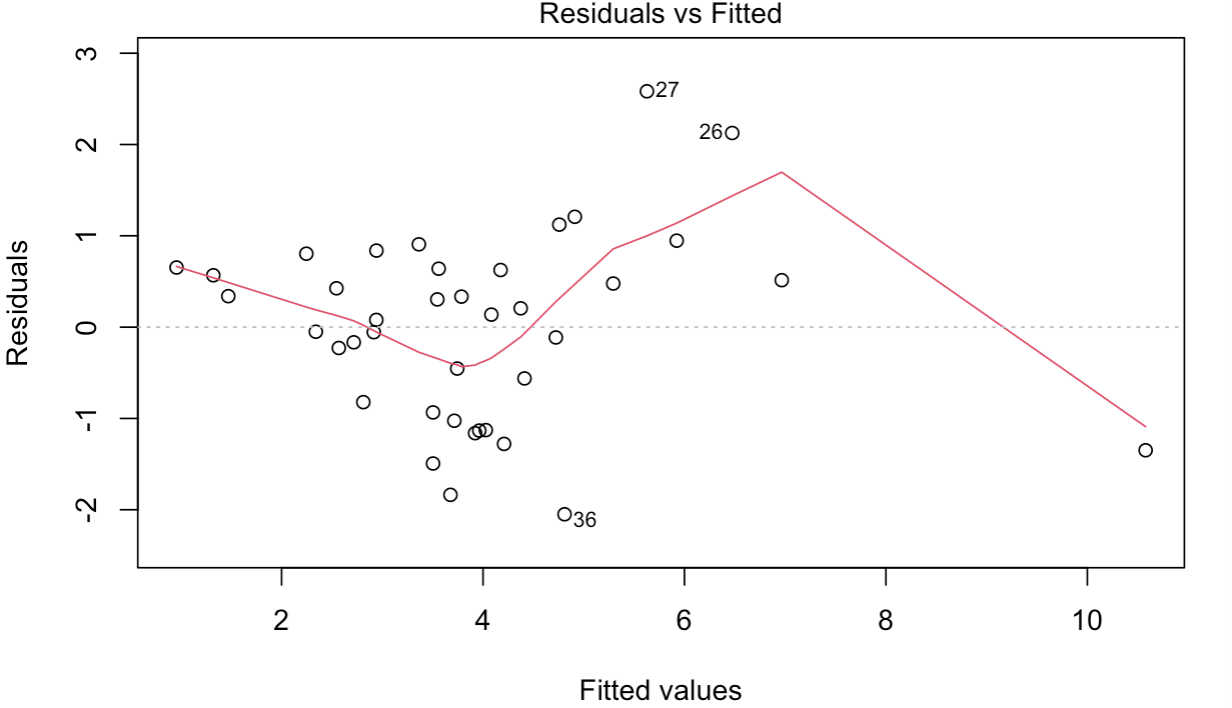
\includegraphics[width=0.8\textwidth]{Adequacy tests/Residual plot.png}
\end{figure}
\noindent

A Box-Cox transformation is performed on the response variable to see if there is a noticeable improvement in the model. Using the "boxcox" function in R a plot for $\lambda$ was created ($\ref{fig:AT2}$) and the $\lambda$ value which maximizes the log-likelihood function was determined to be -0.06060606. The power transfromation with the determined $\lambda$ was applied to the response variable and a new plot of the residuals against the fitted values was produced. Comparing the two plots, the data from the transformed model did appear to make an improvement in the linearity of the plot, as well as deal with some of the issue of increasing variance.

\begin{figure}[H]
    \centering
    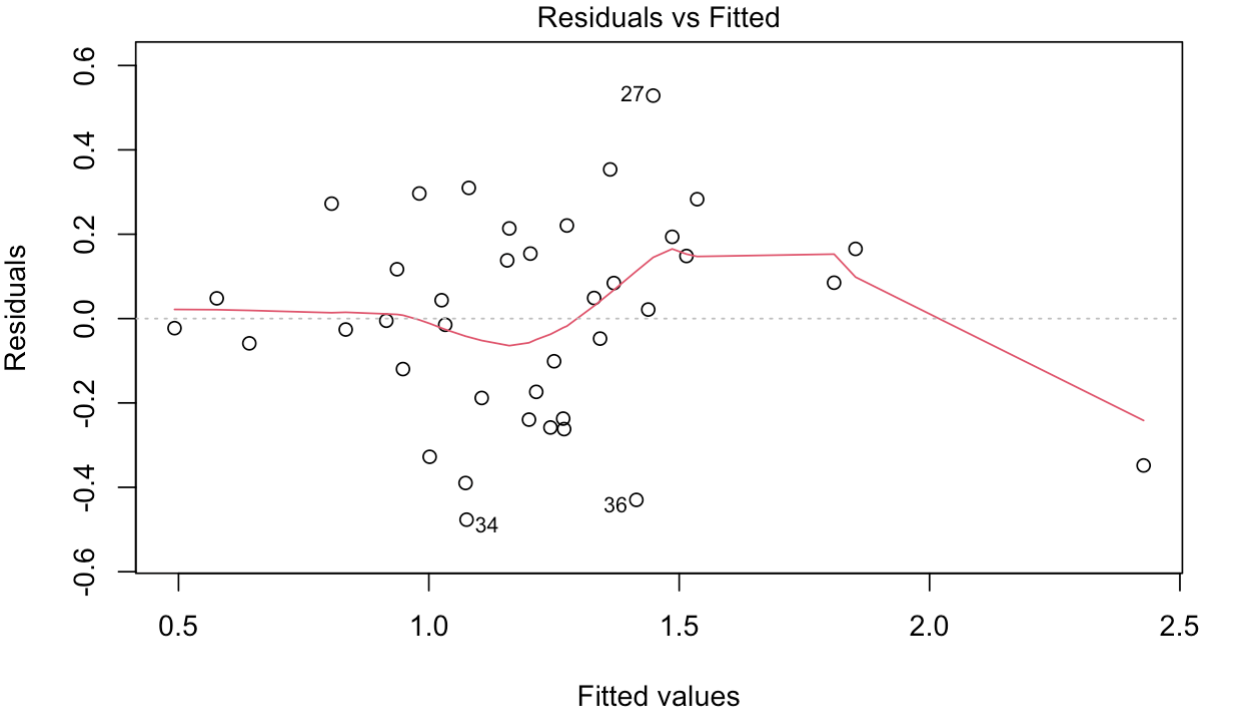
\includegraphics[width=0.8\textwidth]{Adequacy tests/BC plot.png}
\end{figure}
\noindent

Do note that a weighted least squares regression was also constructed for the model. But as can be seen in the new plot there is minimal to no improvement in the linearity of the plot or in the removal of the issue of increasing variance. Thus the Box-Cox transformation is viewed as a better model than the weighted least squares model.

\begin{figure}[H]
    \centering
    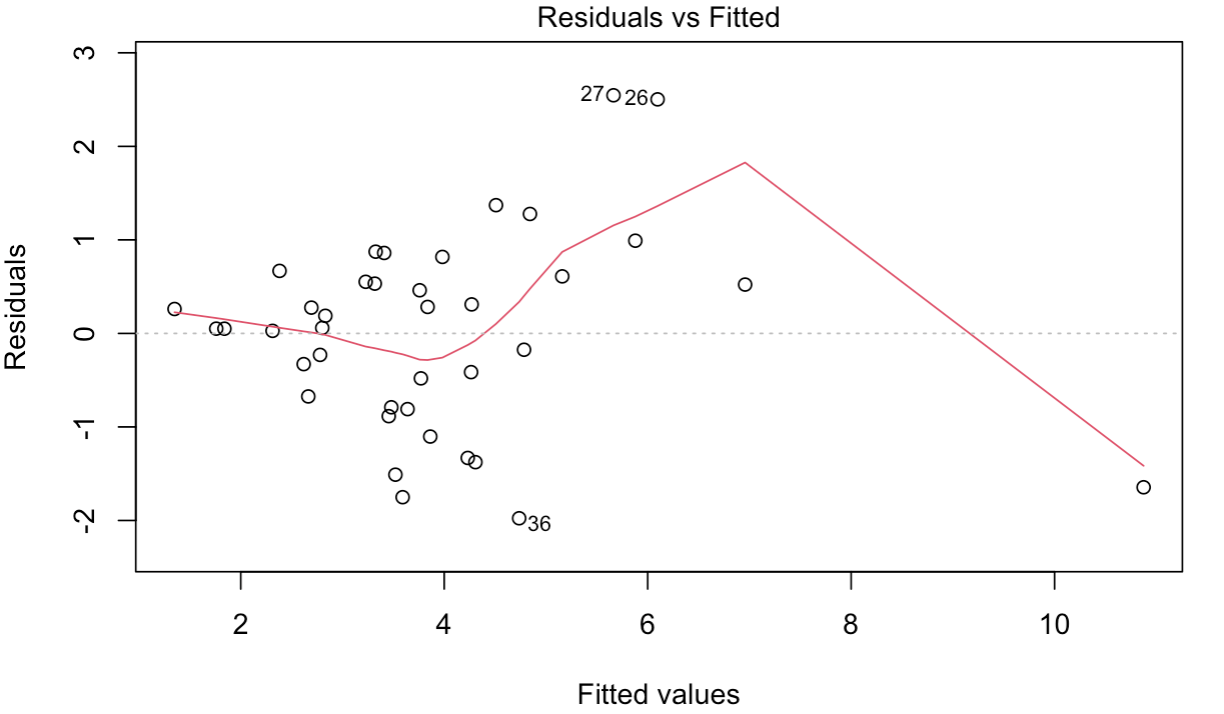
\includegraphics[width=0.8\textwidth]{Adequacy tests/WT plot.png}
\end{figure}
\noindent

Although it appeared that the issue with non constant variance or heteroscedasticity was dealt with during the Box-Cox transformation we verify the assumption by conducting a Breusch-Pagan test on each of the 3 models. With the "bptest" function in R the tests were produced, the results of the tests are summarized below. We see that the p-value for initial the model is 0.1386 > 0.05. Thus we cannot reject the null hypothesis and based on this test there is insufficient evidence to suggest that heteroscedasticity is present in the model, validating our assumption. Unfortunately in looking at the results of the Breusch-Pagan test for the other two models we see that both p-values are much less than 0.05 meaning we would reject the null hypothesis in both cases. Since this is the case there is strong evidence suggesting that there would be an issue with heteroscedasticity if we used either of the two new models, so the original model is kept moving forward.

\begin{table}[H] 
\caption{Breusch-Pagan Test Results} \label{tab:BPtest}
\centering
\begin{adjustbox}{width=0.9\textwidth}
\small
\begin{tabular}{|c|c|c|c|c|}
\hline
{\textbf{Model}} & {\textbf{Observed Test Statistic}} & {\textbf{P-value}} & {\textbf{Decision}} & {\textbf{$R^{2}_{adj}$}} \\ \hline
Initial Model     & 12.293  & 0.1386           & Do not reject $H_{0}$, constant variance & 0.6622 \\ \hline
Box Cox Model     & 16.901 & 0.03116           & Reject $H_{0}$, non-constant variance & 0.6082  \\ \hline
Weighted Least Squares Model     & 31.491 & 0.0001149           & Reject $H_{0}$, non-constant variance & 0.6312  \\ \hline
\end{tabular}
\end{adjustbox}
\end{table}
\noindent

The next assumption we wish to verify is the assumption that the error terms are normally distributed. To do this we construct a normal probability plot of the residuals also referred to as a normal quantile-quantile plot. If they are normally distributed the points will stay on the $45^{\circ}$ dashed line. When dealing with real data it is improbable it will perfectly follow a normal distribution. Since small deviations from the normality assumption do not have a significant impact on the model, we only look for large deviations. As there do not appear to be any departures from the dashed line large enough to violate the normality assumption, we proceed with it. 

\begin{figure}[H]
    \centering
    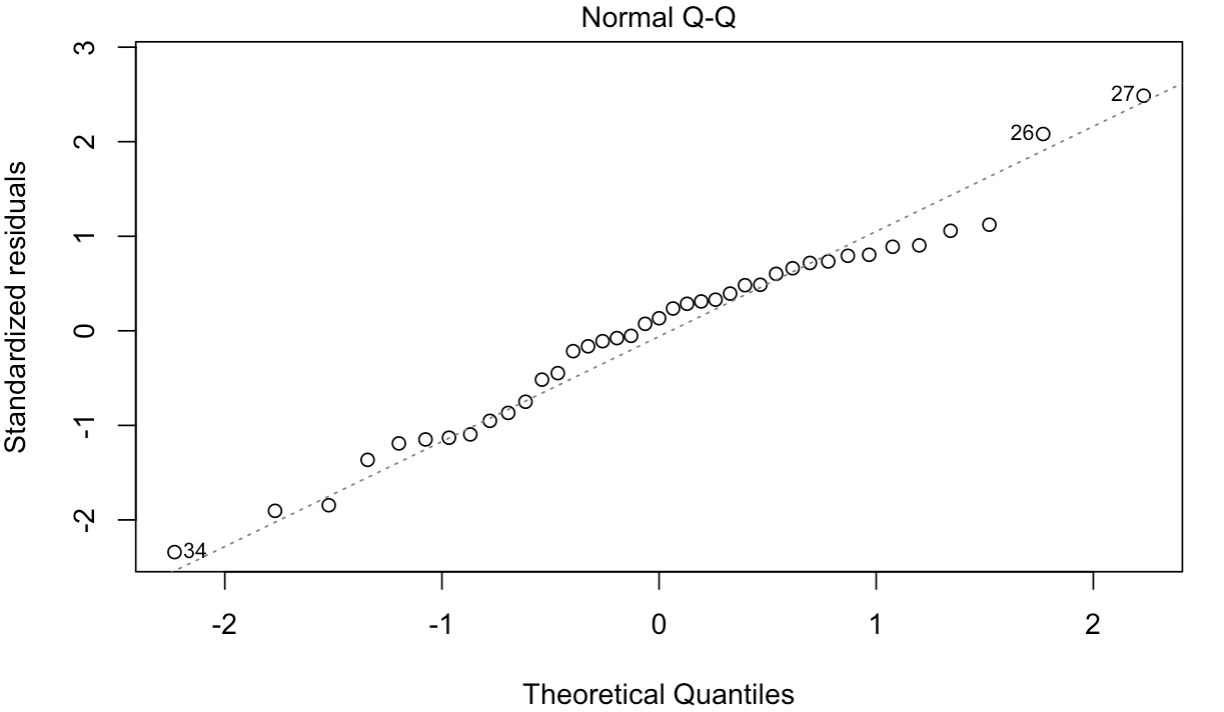
\includegraphics[width=0.8\textwidth]{Adequacy tests/QQ plot.png}
\end{figure}
\noindent

The final check conducted is a verification that the errors are uncorrelated which is done using the Durbin-Watson test. R was used to run the test using the "dwtest" command, according to the results of the test the model has a p-value of 0.8669 which is much greater than 0.05. Consequently we cannot reject the null hypothesis and there is weak evidence to suggest that the correlation of the errors is non zero, assuring our assumption are correct.

Durbin-Watson Test:
\\$H_{0}:$ Correlation of the errors is zero vs $H_{a}:$ Correlation of the errors is non zero
\\$DW = 2.4133$ \quad p-value = 0.8669
\\Decision: Since the p-value is well above the significance level, we do not reject the null hypothesis

\subsection{Variable Selection}
The next step following the completion of the diagnostic and adequacy checking is the variable selection in which we will find the appropriate subset of regressors for the model. Multiple linear regression models often use variables that do not have a relationship with the response variable of interest. As a result, including these irrelevant features is likely to complicate the model and degrade its performance. Subset selection is used to aid in the selection of relevant predictors related to the response.

Because the number of predictors in the full model is small an exhaustive search for the best subset was conducted which selects the best model out of the $2^p$ possibilities of model construction. Figure \ref{fig:VS1} shows a summary of the best subset models where an asterisk indicates that a given variable is included in the corresponding model. The presence of more asterisks indicates that a variable is more significant and as such we see that the number of access points and the length of the highway are the two most significant variables in the regression.

In the case of a collection of models with different numbers of predictors, $R^2$ is not suitable for selecting the best model since a model containing all of the predictors will always have the largest $R^2$. Mallow's $C_{p}$ and adjusted $R^2$ are used instead as they take into account the number of parameters in the model. Two plots (\ref{fig:VS2}, \ref{fig:VS3}) were constructed showing of the variables present in the best subset models ranked according to adjusted $R^2$ and Mallow's $C_{p}$. The top row of each plot contains a black square for each variable included in the most optimal model according to each statistic. Based on the plot using adjusted $R^2$ as the scale the best subset of predictors includes the number of access points, the highway length, the speed limit, and the truck volume. The plot using Mallow's $C_{p}$ indicates the optimal subset of predictors includes only the number of access points, the highway length, and the speed limit. 

Based on the results of these two plots the recommended subset model is to include the four predictors identified in the adjusted $R^2$ plot yielding the new equation 
\begin{equation} \label{bestEq}
    \begin{aligned}
    \hat{y} = 10.1711 - 0.09848x_{3} + 0.09476x_{5} - 0.12877x_{6} - 0.05988x_{8}
    \end{aligned}
\end{equation}

\subsection{Hypothesis Tests}

Once the fitted model was obtained and all diagnostic and adequacy checks were completed hypothesis tests could be undertaken to determine the statistical significance of the regression model as a whole as well as the individual parameters. The summary and anova commands in R are used to calculate the observed t and F values and their corresponding p-values for each of the parameters. All data used in the following hypothesis tests can be found in figure (\ref{fig:HT2}).    

Test on Speed Limit Parameter:
\\$H_{0}: \hat{\beta_{3}} = 0$ vs $H_{a}: \hat{\beta_{3}} \neq 0$
\\$t_{obs} = -2.319$ \quad p-value = 0.0265
\\Decision: Since the p-value is below the significance level of 0.05, we reject the null hypothesis and so the evidence suggests that the speed limit has statistical significance on accident rates.

Test on Number of Access Points Parameter:
\\$H_{0}: \hat{\beta_{5}} = 0$ vs $H_{a}: \hat{\beta_{5}} \neq 0$
\\$t_{obs} = 3.467$ \quad p-value = 0.0014
\\Decision: Since the p-value is well below the significance level, we reject the null hypothesis and there is strong evidence suggesting that the number of access points is statistically significant.

Test on Truck Volume Parameter:
\\$H_{0}: \hat{\beta_{6}} = 0$ vs $H_{a}: \hat{\beta_{6}} \neq 0$
\\$t_{obs} = -1.389$ \quad p-value = 0.1740
\\Decision: Because the p-value is clearly above 0.05, we cannot reject the null hypothesis and as a result of not rejecting the null hypothesis, the evidence indicates little statistical significance associated with a truck volume on accident rates.

Test on Highway Length Parameter:
\\$H_{0}: \hat{\beta_{8}} = 0$ vs $H_{a}: \hat{\beta_{8}} \neq 0$
\\$t_{obs} = -2.177$ \quad p-value = 0.0365
\\Decision: Given the p-value is below 0.05, we reject the null hypothesis and claim there is strong evidence supporting that the highway length is statistically significant.

Test on Regression Model:
\\$H_{0}: \hat{\beta_{1}} = \hat{\beta_{2}} = ... =\hat{\beta_{8}} = 0$ vs $H_{a}: \text{at least one }\hat{\beta_{j}} \neq 0$
\\$F_{obs} = 21.52$ \quad p-value = $6.373 \times 10^{-9}$
\\Decision: Given the p-value corresponding to the observed F value is well below 0.05, we reject the null hypothesis and claim there is strong evidence supporting that at least one of $\hat{\beta_{j}} \neq 0$ and that the regression model is statistically significant.
\bigskip

We can conclude from the above tests that the fitted regression model is significant, meaning there exists a linear relationship between the response variable and the regressor variables. Only the truck volume was deemed not relevant in predicting the collision rate on highways. Thus the variables that showed a linear relationship with the accident rate were the number of access points, the length of the highway, and the speed limit. Where the number of access points demonstrated a positive effect, the length of the highway and speed limit demonstrate negative effects.

\chapter{Discussion}
Using the data taken from the data set \textit{Highway1} \cite{Data} and the many packages available in R, this study was able to address the problem of how to reduce accident rates on highways. 

The first step in the analysis was conducting a check for outliers, high leverage and influential observations. The tests indicated no outliers were present in the data but identified that 4 values in the data could be classified as high leverage points, observations 1, 2, 25, and 34. Since each of these data points were deemed to not be of high influence no data points needed to be removed and it was safe to proceed with the analysis. In the following step, we tested for multicollinearity three ways and all agreed with each other that no multicollinearity existed between the variables. 

In order to assess the suitability of the original fitted model, an adequacy test was performed. In order to test the adequacy of the model certain assumptions needed to be verified, linearity between response and regressor variables and the model needed to possess an error term that was uncorrelated and approximately normally distributed with constant variance. The Durbin-Watson test showed that there is weak evidence to suggest that the correlation of the errors is non zero, allowing us to assume they are uncorrelated. To verify the assumption of normally distributed error a normal quantile-quantile plot was constructed. Since there did not appear to be any large departures from the $45^{\circ}$ dashed line the normality assumption also holds. A plot of the residuals against the fitted values appear to take on an outward opening funnel pattern with a trend line that was non linear. This indicates non linearity as well as non-constant variance, which contradicted the Breusch-Pagan test that determined there is insufficient evidence to suggest that heteroscedasticity is present in the model. To help remedy this both a Box-Cox transformation and weighted least squares regression were both applied. Unfortunately in both cases the $R_{j}^2$ values decreased from the initial model falling from 0.6622 to 0.6082 for the Box-Cox model and to 0.6312 for the weighted least squares model. Additionally conducting Breusch-Pagan tests on the two new models displayed non-constant error terms. As a result neither of the new models showed an improvement from the original model so the original model was taken moving forward.   

Since multiple linear regression models often use irrelevant variables that do not have a relationship with the response variable of interest we attempted to determine the best subset of variables that accurately explain the data. To ascertain the best model from the $2^p = 512$ possible combinations we ranked each of the models by their respective $R_{j}^2$ and Mallow's $C_{p}$ values. These rankings yielded differing results, with the best model with respect to Mallow's $C_{p}$ being one including the number of access points, the highway length, and the speed limit. The optimal model proposed by the $R_{j}^2$ ranking included the truck volume in addition to the three variables in the other ranking. As such the model containing four variables was taken moving forward as the best model, transitioning from the original model to the new 4 variable model increased the $R_{j}^2$ by 2$\%$.

Hypothesis tests conducted on the optimal model showed that the truck volume was the only variable to be not statistically significant in predicting the accident rate. Based on equation $\eqref{bestEq}$ we see that the intercept is 10.17 but since this would be when each of the regressor variables is zero to get the base accident rate we take the value produced when each of the variables are at a minimum. This value is 6.244 meaning the base accident rate is a little above 6$\%$ per million vehicle miles. The number of access points demonstrates a positive effect on accident rate, meaning that as the number of on ramps a highway possessed increases so does the number of collisions occuring. This makes sense as not every driver has the skill and experience necessary to execute safe merges onto a highway. We see that the speed limit actually shows a negative relationship with accident rate which is unexpected as the faster a car is travelling the less time the driver has to react to situations. Similarily as the highway length increases we expect a decrease in the collision rate. 

The uneven spread in the data for some of the predictor variables may have cause some issues of appeared non-linearity and non constant variance seen in the plot of the residuals versus fitted values possibly effecting the reliability of the model. Looking past that as a whole this analysis presents a model that does a reasonably well job of fitting to the data given an $R_{j}^2$ value of 0.6835. As a result governments can use the insights provided by this model to optimize the design and construction of new highways to reduce crash rates. 


\begin{thebibliography}{9}
\bibitem{Gov}
Rzeznikiewiz D, Tamim H, Macpherson AK (2012) 
\textit{Risk of death in crashes on Ontario’s highways}.
BMC Public Health 12: 1125.

\bibitem{Data}
Fox J, and Weisberg S, (2019) 
\textit{An R Companion to Applied Regression}. 
Third Edition. Sage.

\end{thebibliography}

\chapter{Appendices}
\section{Supplementary Tables and Figures}
\begin{figure}[H]
    \centering
    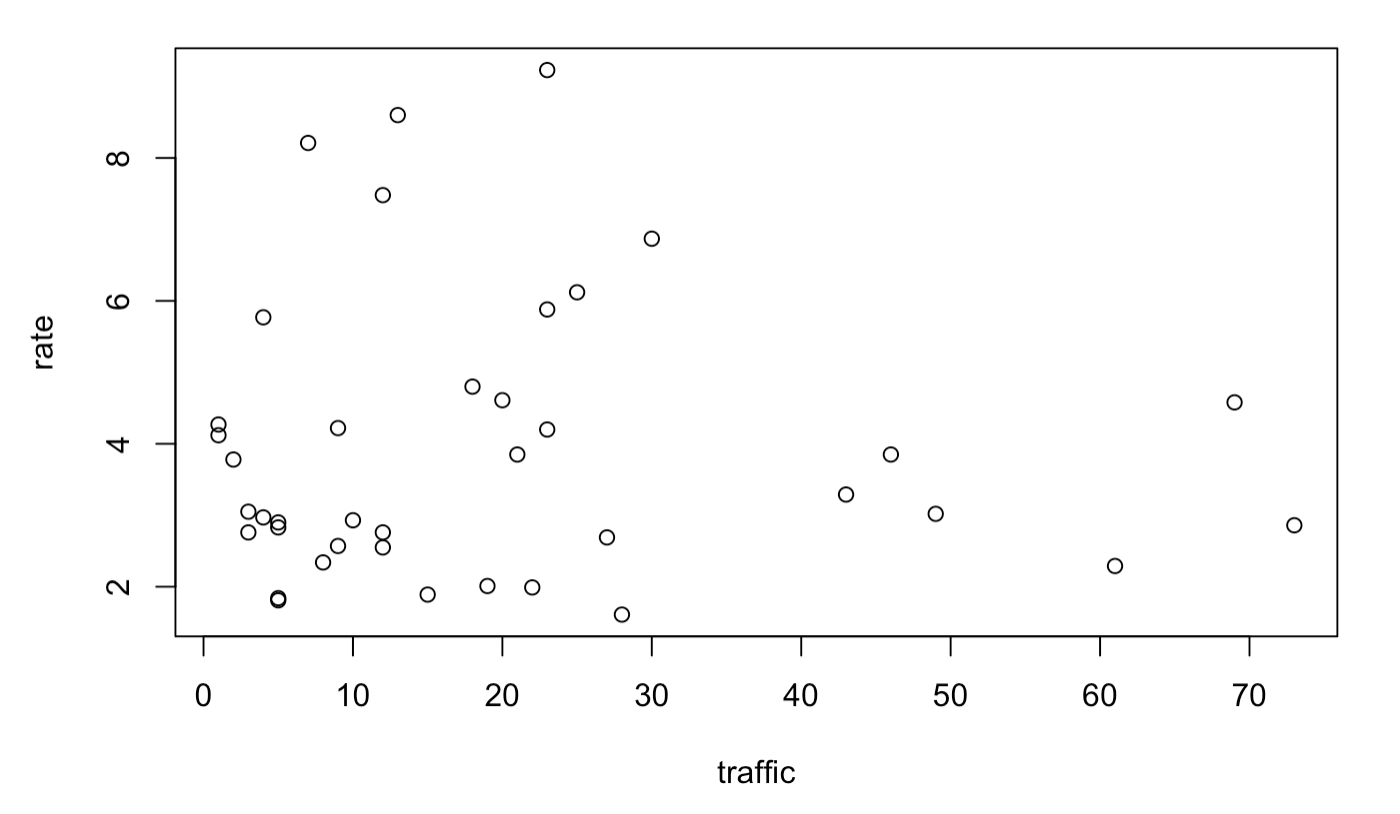
\includegraphics[width=1\textwidth]{Preliminary graphs/ST562 Rate vs Traffic.png}
    \caption{Collision Rate versus Traffic Volume} \label{fig:PG1}
\end{figure}
\noindent

\begin{figure}[H]
    \centering
    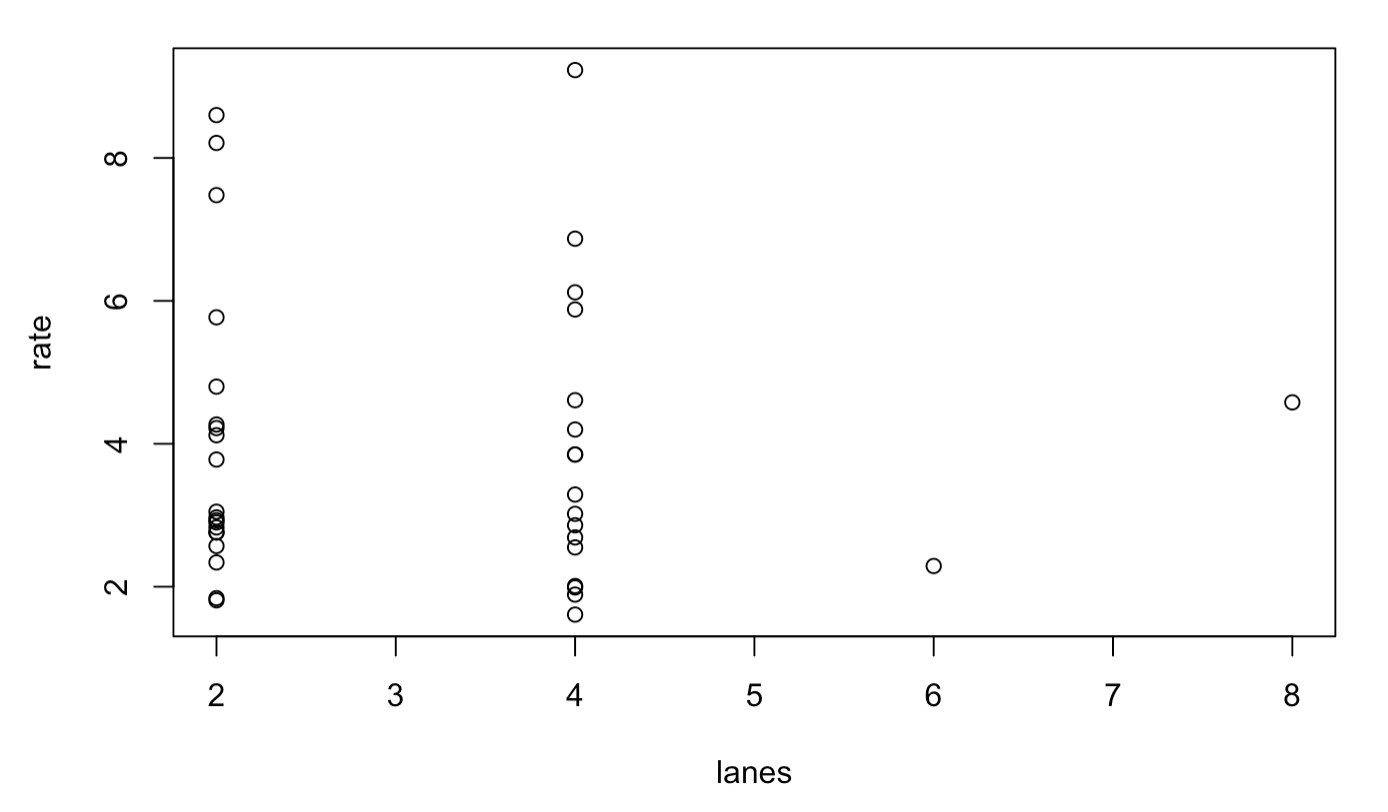
\includegraphics[width=1\textwidth]{Preliminary graphs/ST562 rate vs lanes.png}
    \caption{Collision Rate versus Lane Number} \label{fig:PG2}
\end{figure}
\noindent

\begin{figure}[H]
    \centering
    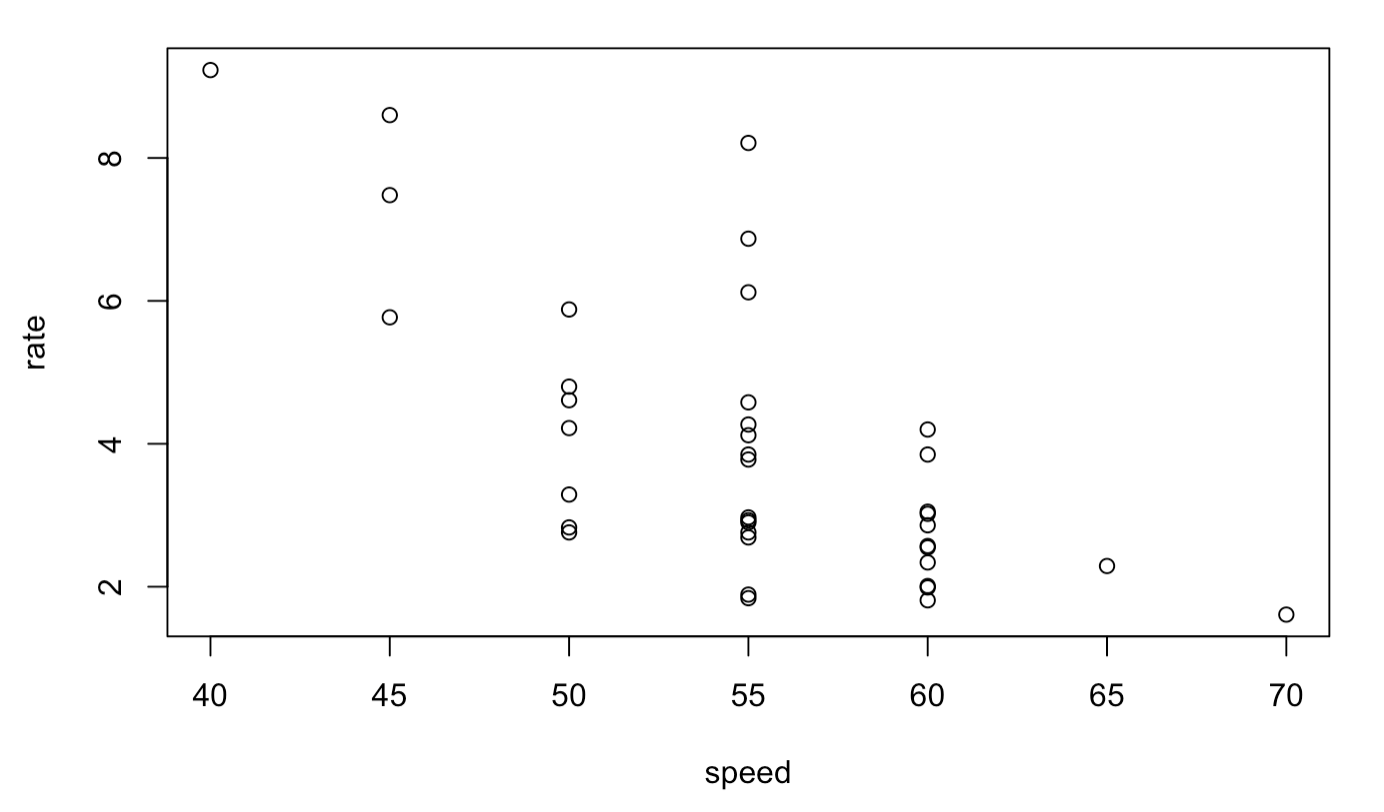
\includegraphics[width=1\textwidth]{Preliminary graphs/ST562 rate vs speed.png}
    \caption{Collision Rate versus Speed Limit} \label{fig:PG3}
\end{figure}
\noindent

\begin{figure}[H]
    \centering
    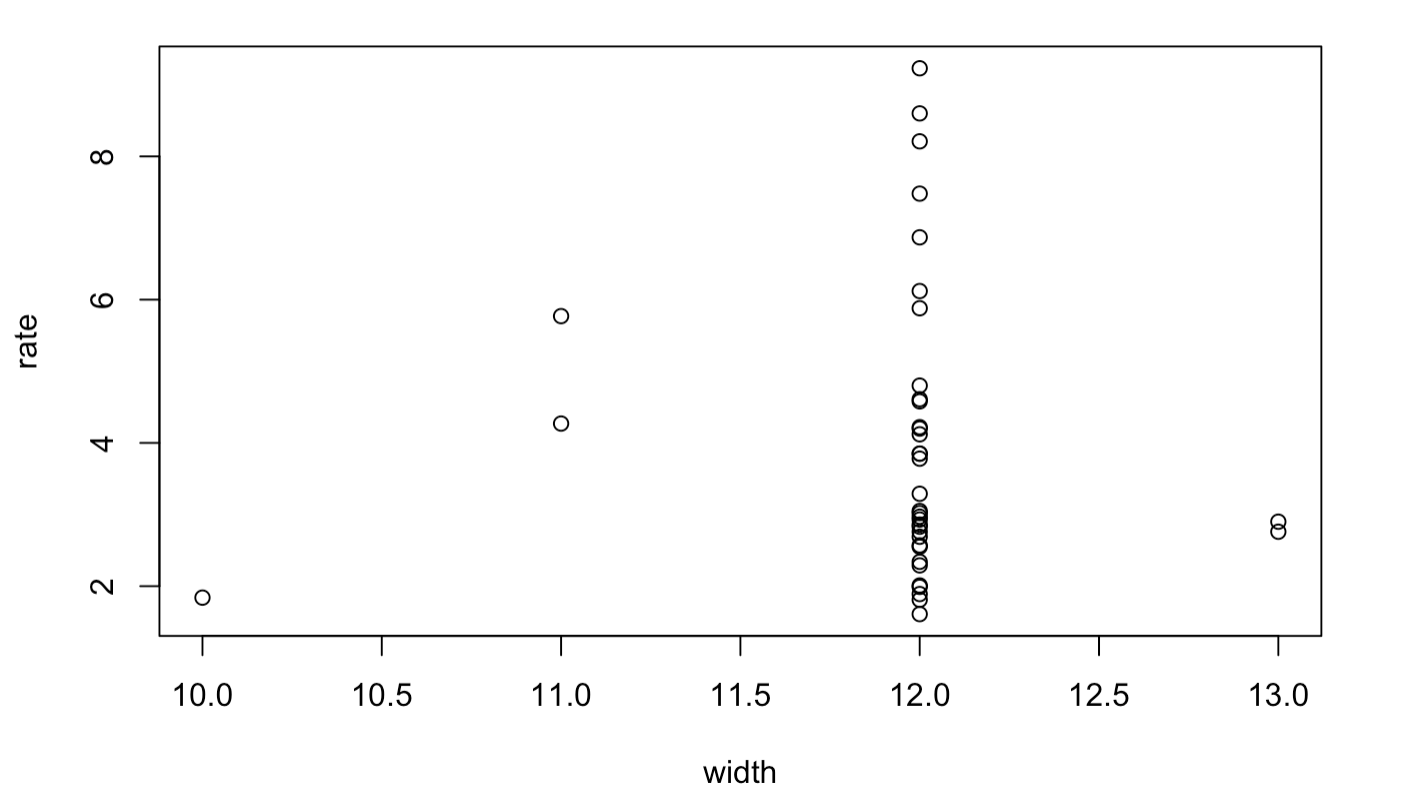
\includegraphics[width=1\textwidth]{Preliminary graphs/ST562 rate vs width.png}
    \caption{Collision Rate versus Lane Width} \label{fig:PG4}
\end{figure}
\noindent

\begin{figure}[H]
    \centering
    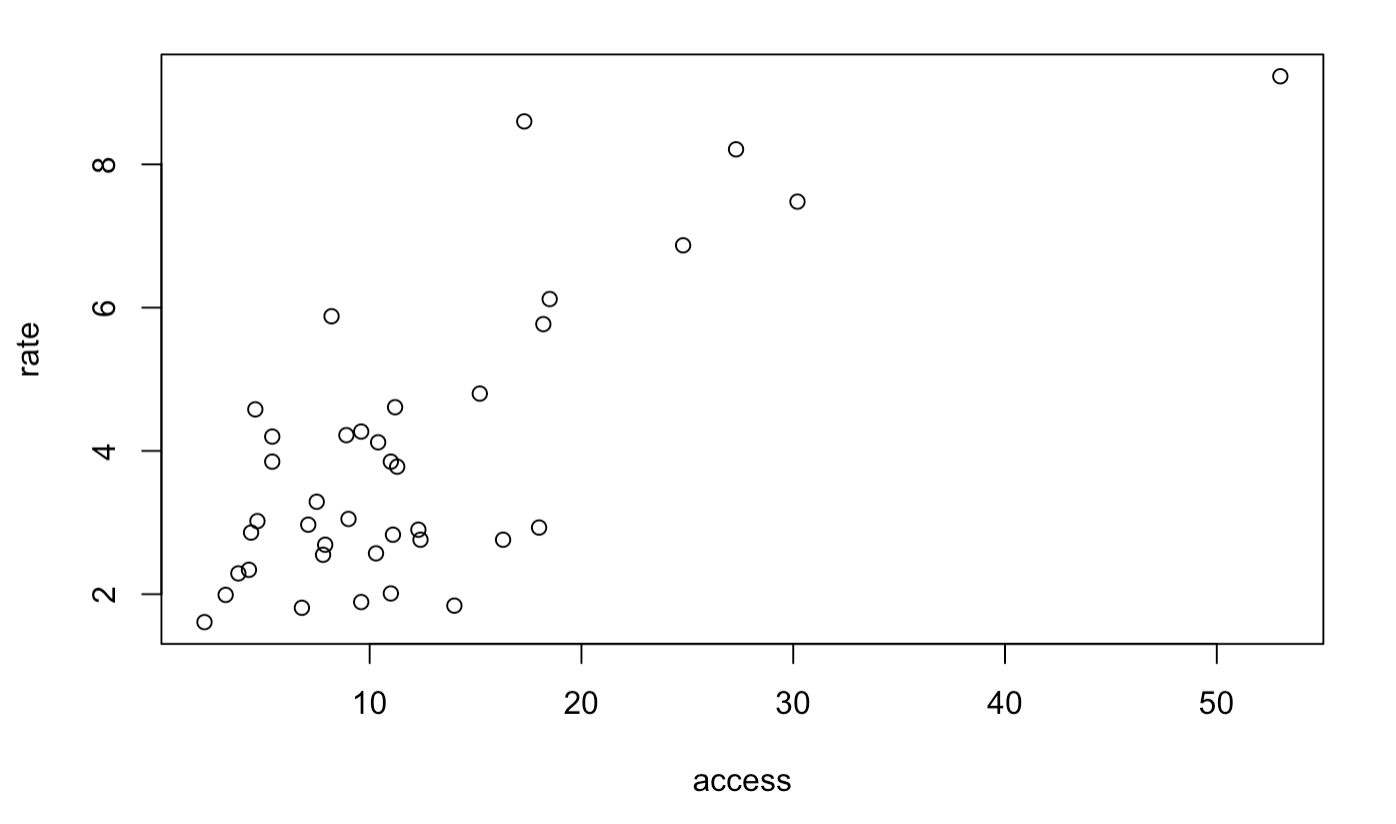
\includegraphics[width=1\textwidth]{Preliminary graphs/ST562 rate vs access.png}
    \caption{Collision Rate versus Access Points} \label{fig:PG5}
\end{figure}
\noindent

\begin{figure}[H]
    \centering
    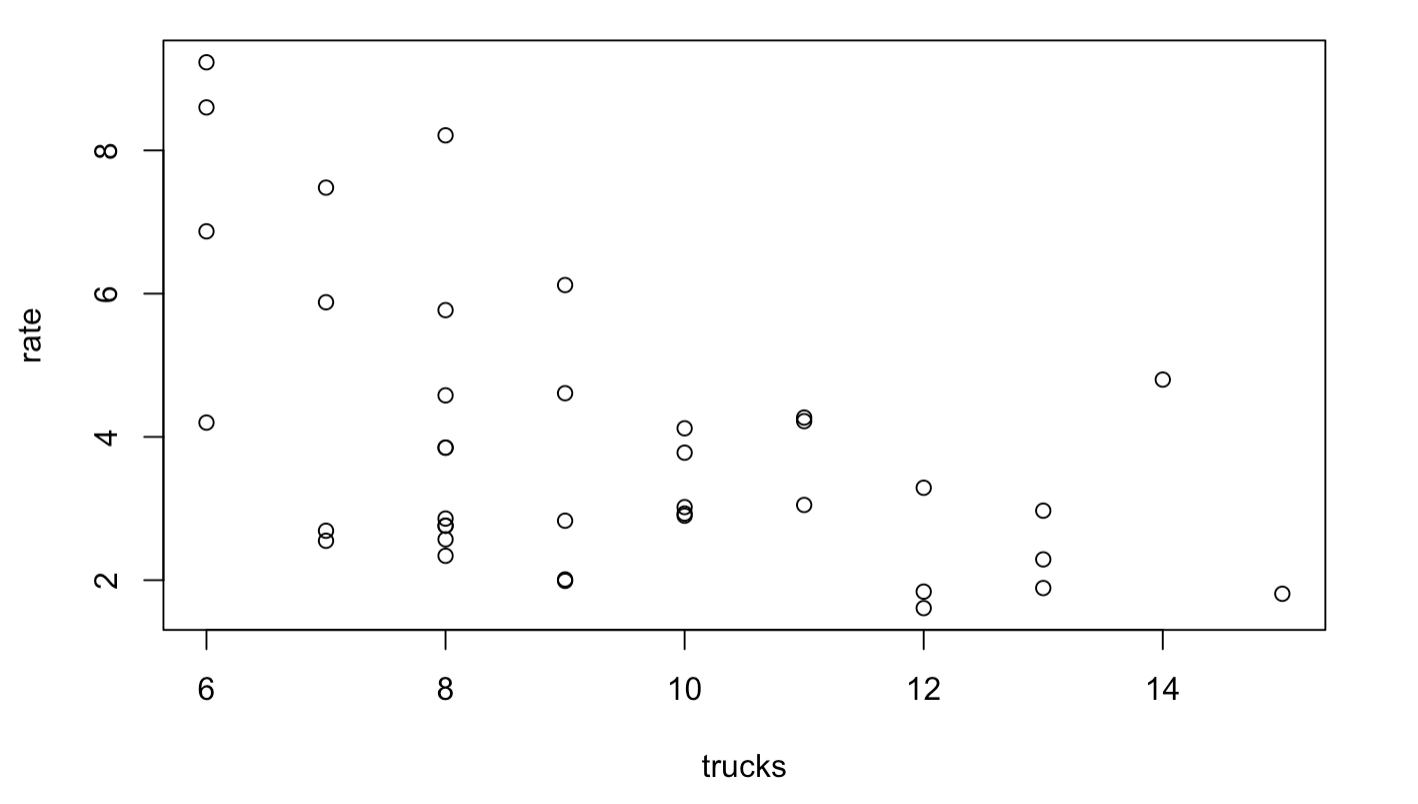
\includegraphics[width=1\textwidth]{Preliminary graphs/ST562 rate vs trucks.png}
    \caption{Collision Rate versus Truck Volume} \label{fig:PG6}
\end{figure}
\noindent

\begin{figure}[H]
    \centering
    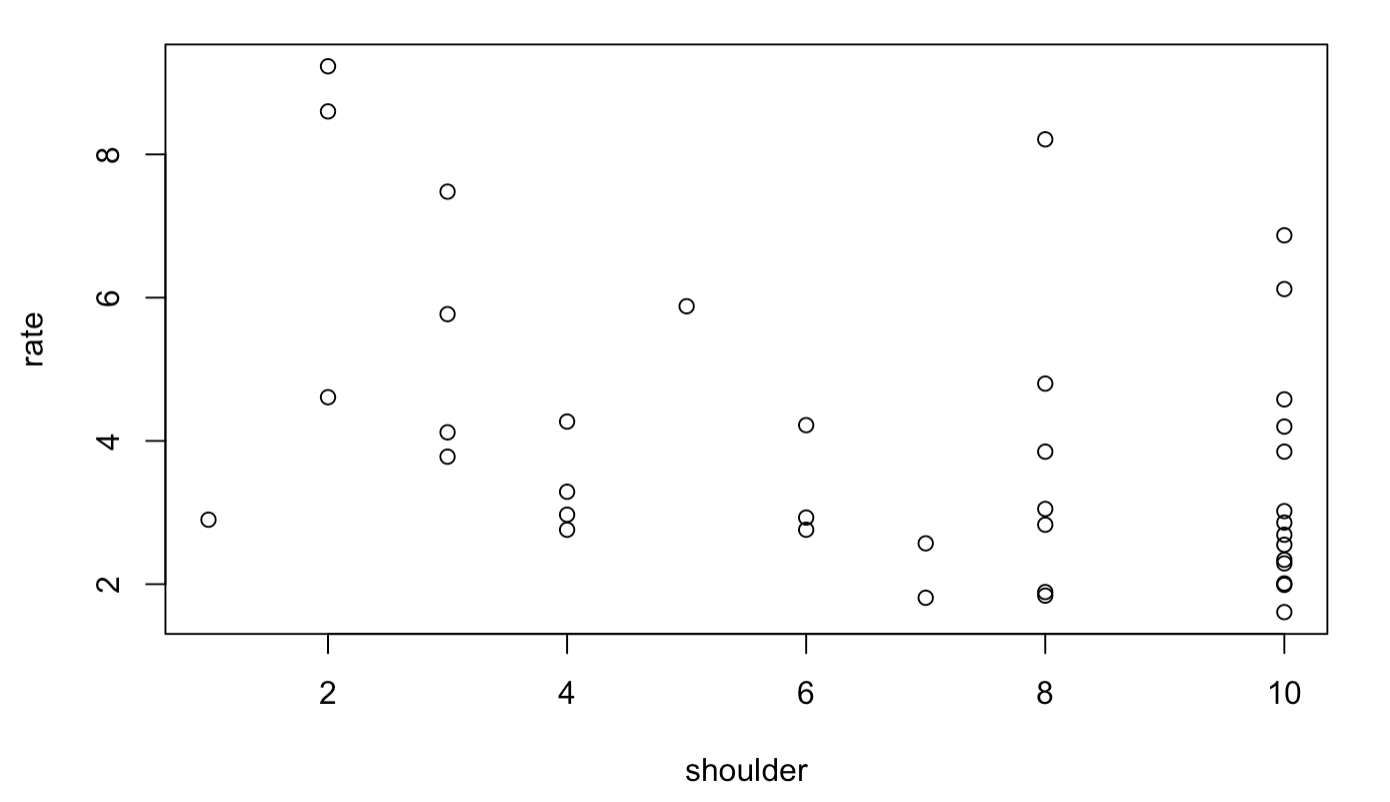
\includegraphics[width=1\textwidth]{Preliminary graphs/ST562 rate vs shoulder.png}
    \caption{Collision Rate versus Shoulder Width} \label{fig:PG7}
\end{figure}
\noindent

\begin{figure}[H]
    \centering
    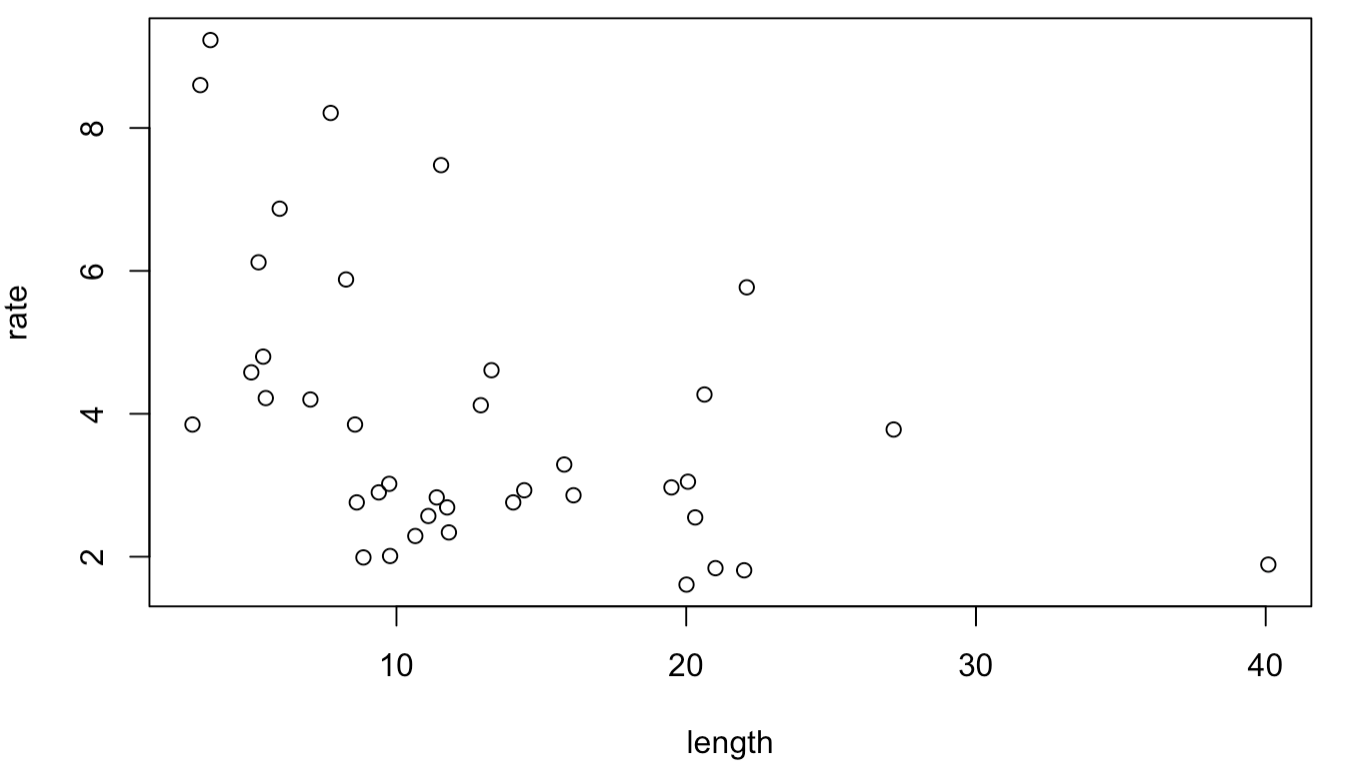
\includegraphics[width=1\textwidth]{Preliminary graphs/ST562 Rate vs Length.png}
    \caption{Collision Rate versus Highway Length} \label{fig:PG8}
\end{figure}
\noindent

\begin{figure}[H]
    \centering
    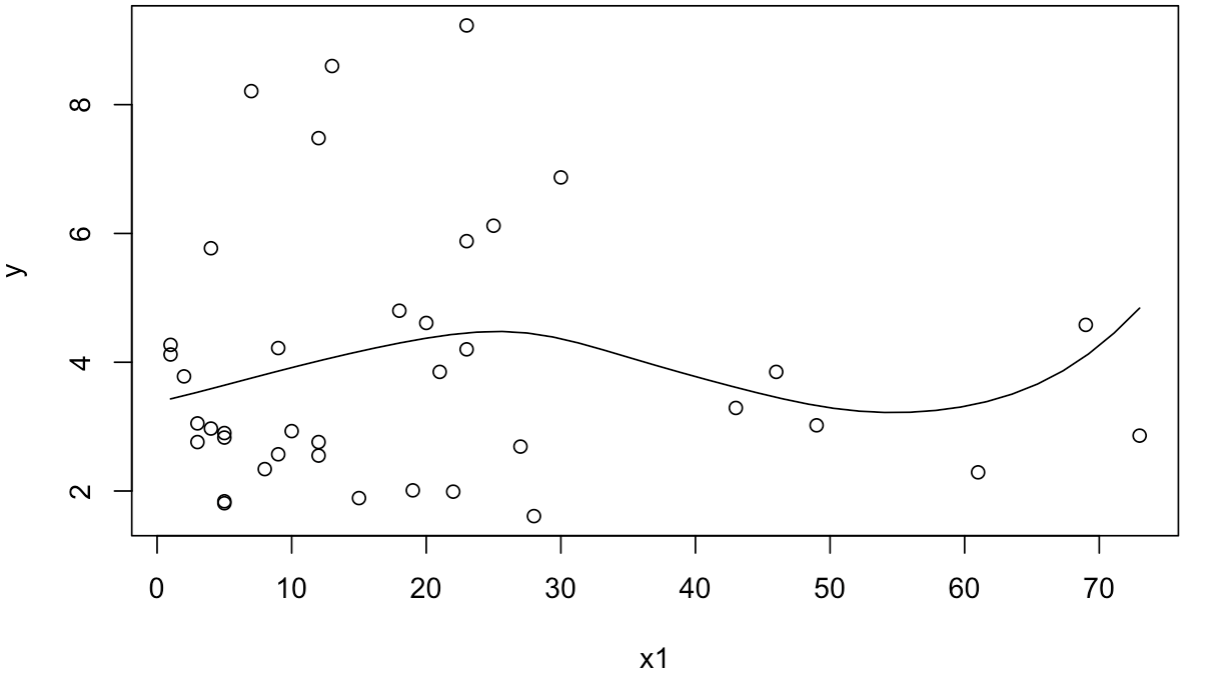
\includegraphics[width=1\textwidth]{Non-parametric/Non-para x1.png}
    \caption{Non-parametric modelling of Collision Rate versus Traffic Volume} \label{fig:NP1}
\end{figure}
\noindent

\begin{figure}[H]
    \centering
    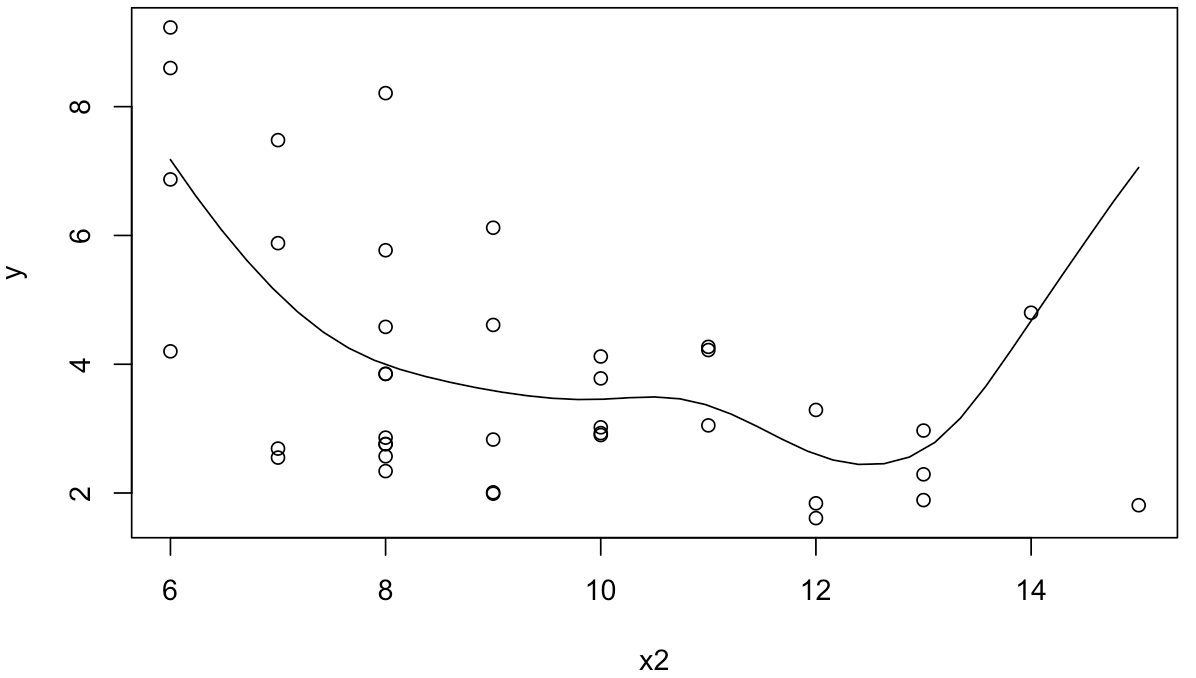
\includegraphics[width=1\textwidth]{Non-parametric/Non-para x2.png}
    \caption{Non-parametric modelling of Collision Rate versus Lane Number} \label{fig:NP2}
\end{figure}
\noindent

\begin{figure}[H]
    \centering
    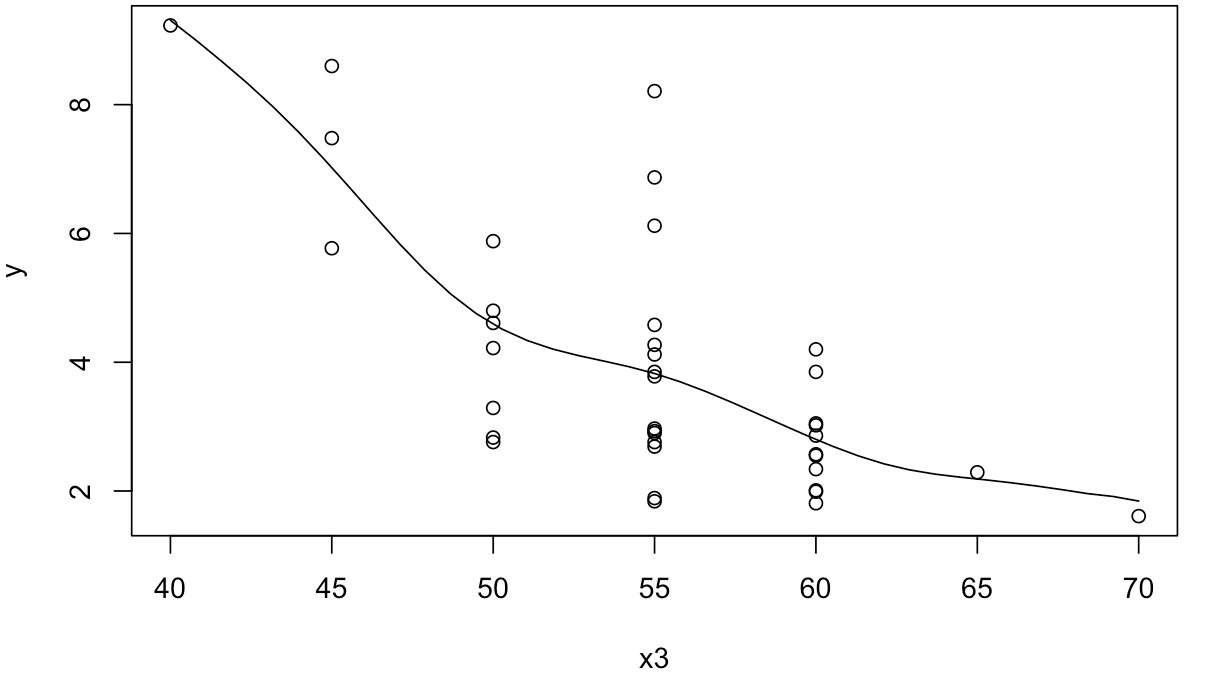
\includegraphics[width=1\textwidth]{Non-parametric/Non-para x3.png}
    \caption{Non-parametric modelling of Collision Rate versus Speed Limit} \label{fig:NP3}
\end{figure}
\noindent

\begin{figure}[H]
    \centering
    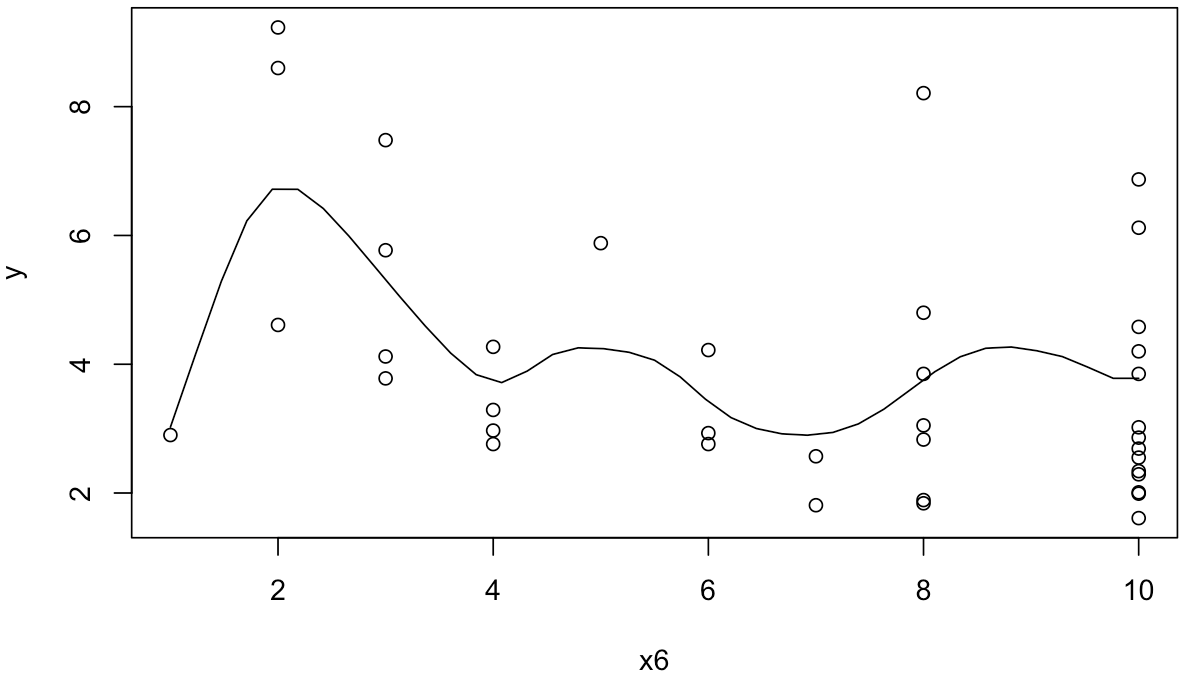
\includegraphics[width=1\textwidth]{Non-parametric/Non-para x6.png}
    \caption{Non-parametric modelling of Collision Rate versus Truck Volume} \label{fig:NP6}
\end{figure}
\noindent

\begin{figure}[H]
    \centering
    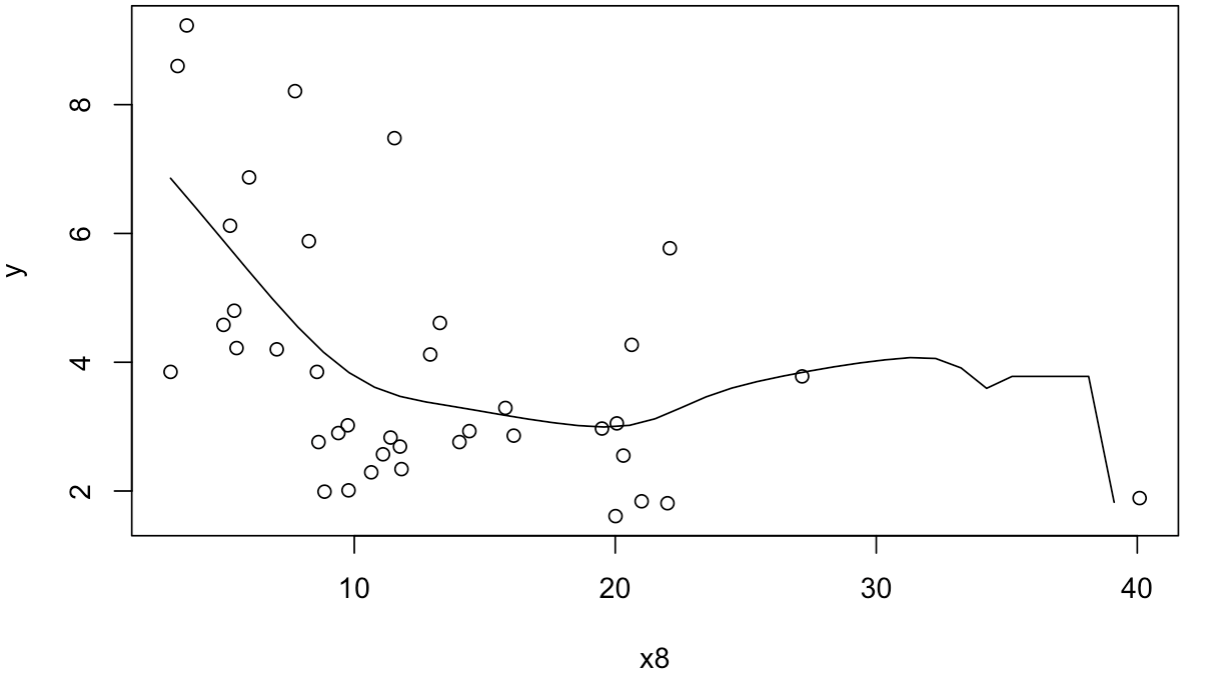
\includegraphics[width=1\textwidth]{Non-parametric/Non-para x8.png}
    \caption{Non-parametric modelling of Collision Rate versus Highway Length} \label{fig:NP8}
\end{figure}
\noindent

\begin{figure}[H]
    \centering
    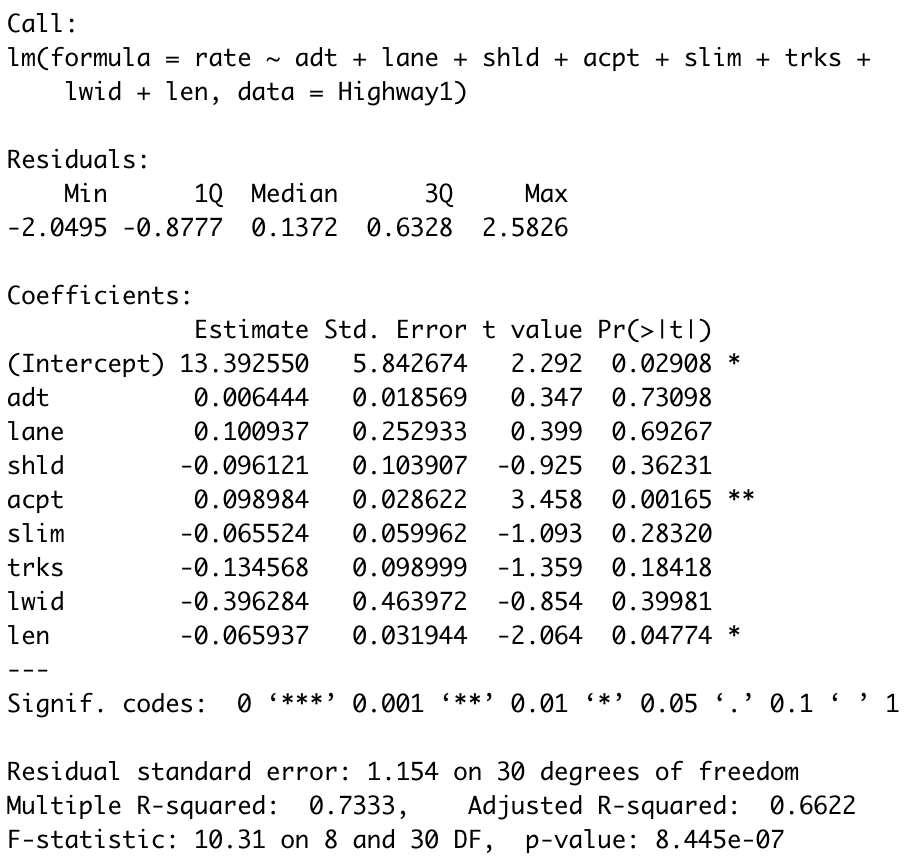
\includegraphics[width=0.65\textwidth]{Hypothesis tests/ST562 Full Model Sum.png}
    \caption{Summary of Full Regression Model} \label{fig:HT1}
\end{figure}
\noindent

\begin{figure}[H]
    \centering
    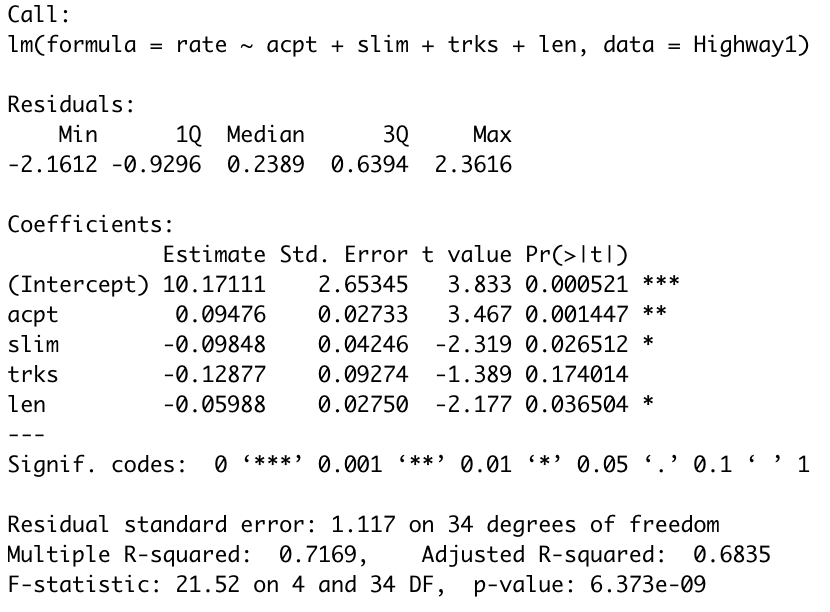
\includegraphics[width=0.65\textwidth]{Variable Selection/Summary Final Model.png}
    \caption{Summary of Final Regression Model} \label{fig:HT2}
\end{figure}
\noindent

\begin{figure}[H]
    \centering
    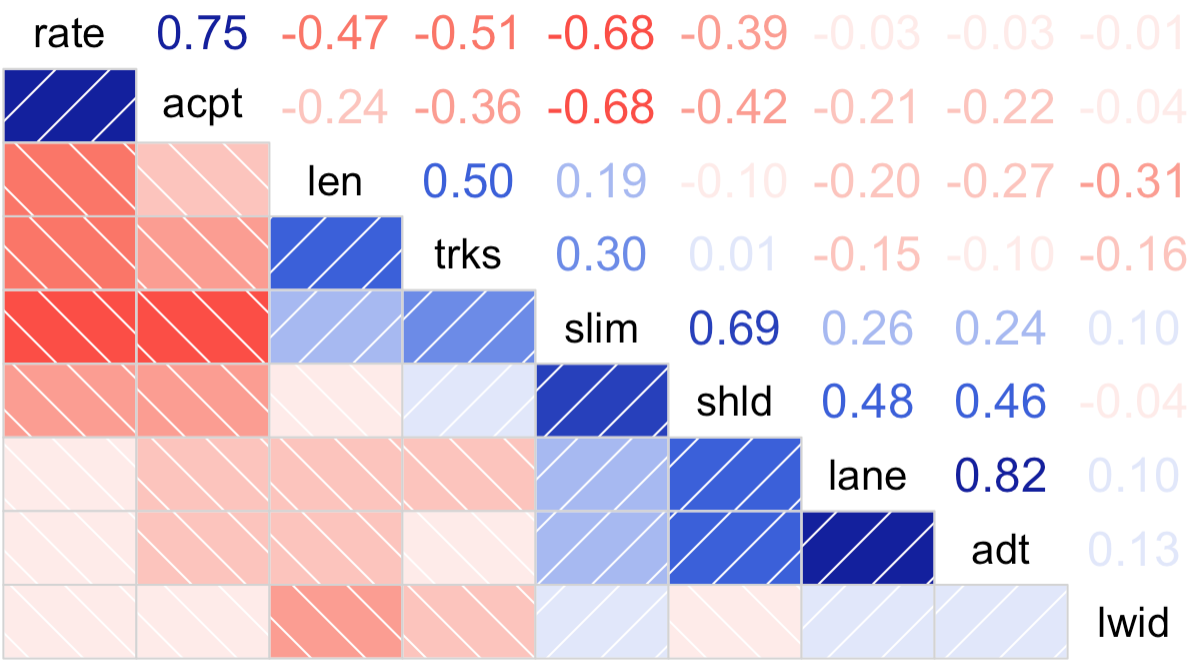
\includegraphics[width=0.8\textwidth]{Diagnostics/ST562 Corr Matrix.png}
    \caption{Correlation Matrix of Highway1 Data} \label{fig:DC1}
\end{figure}
\noindent

\begin{figure}[H]
    \centering
    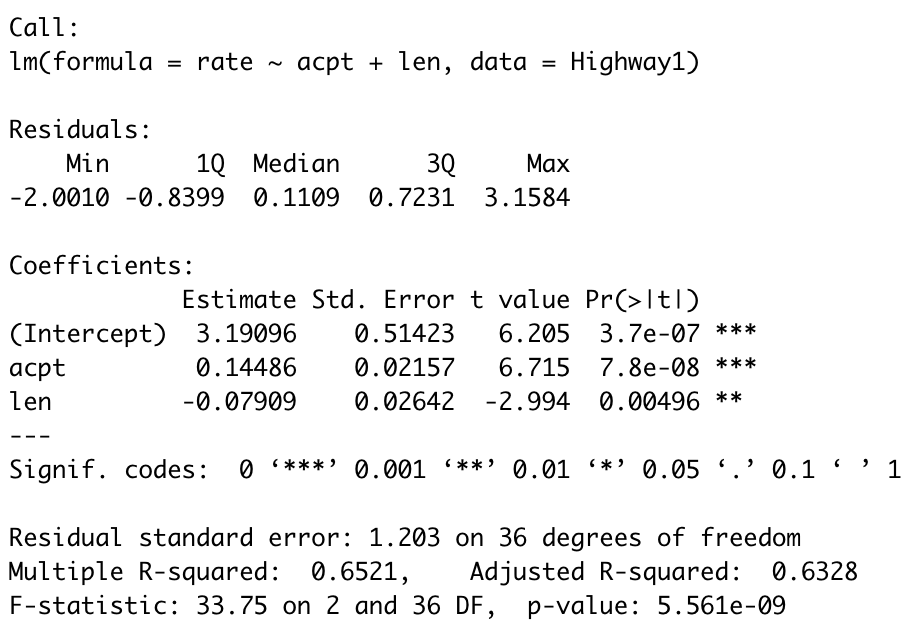
\includegraphics[width=0.65\textwidth]{Hypothesis tests/Reduced model.png}
    \caption{Summary of Reduced Regression Model} \label{fig:HT3}
\end{figure}
\noindent

\begin{figure}[H]
    \centering
    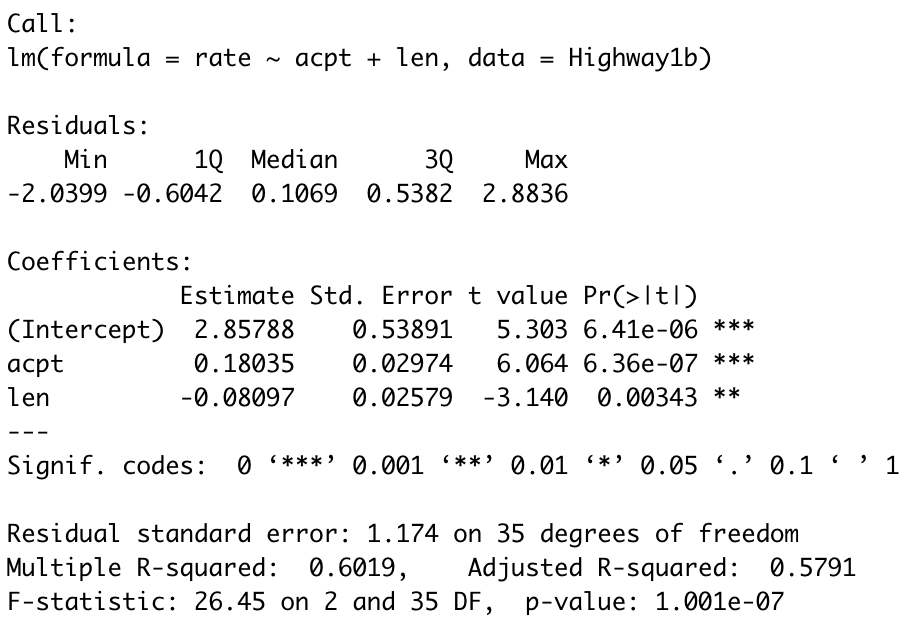
\includegraphics[width=0.65\textwidth]{Diagnostics/Reduced model 2.png}
    \caption{Summary of Reduced Model After Removal of Influential Point} \label{fig:DC2}
\end{figure}
\noindent

\begin{figure}[H]
    \centering
    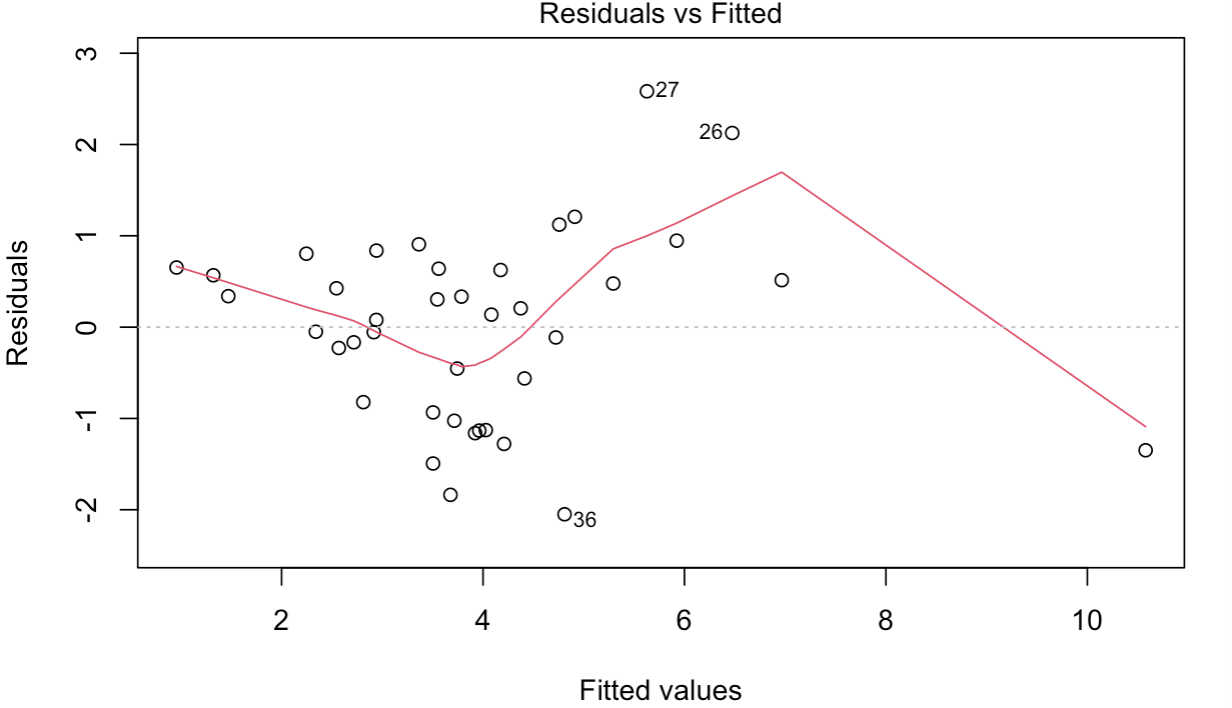
\includegraphics[width=1\textwidth]{Adequacy tests/Residual plot.png}
    \caption{Plot of Residuals Against Fitted Values} \label{fig:AT1}
\end{figure}
\noindent

\begin{figure}[H]
    \centering
    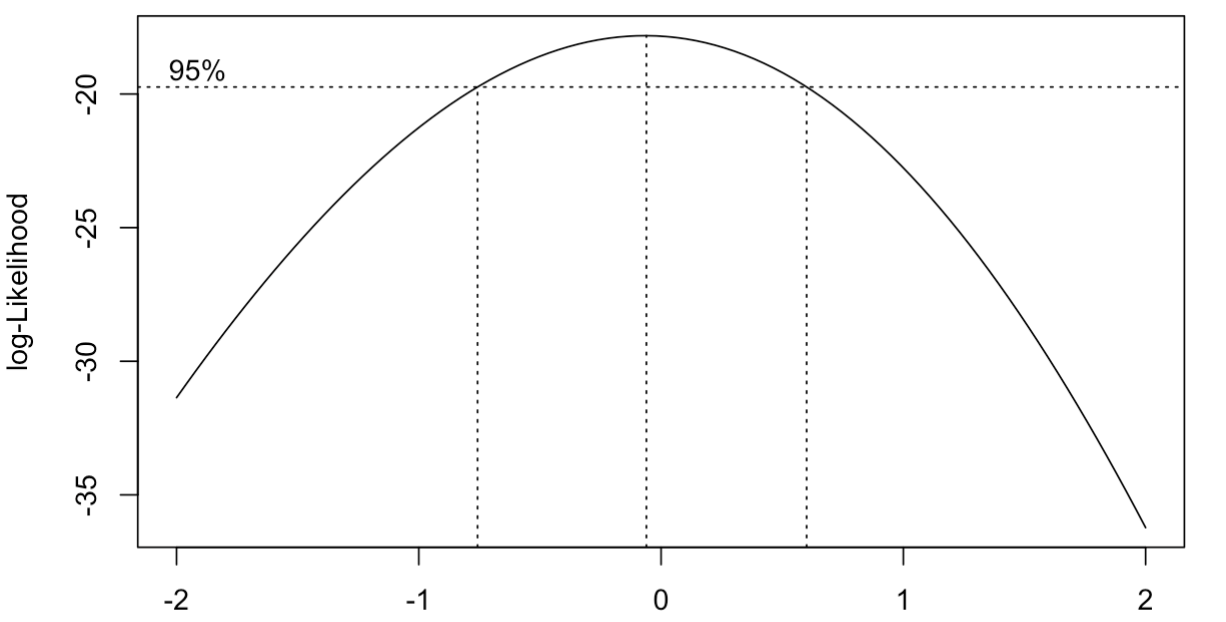
\includegraphics[width=1\textwidth]{Adequacy tests/Boxcox.png}
    \caption{Plot to Determine $\lambda$ That Maximizes the Log-likelihood Function} \label{fig:AT2}
\end{figure}
\noindent

\begin{figure}[H]
    \centering
    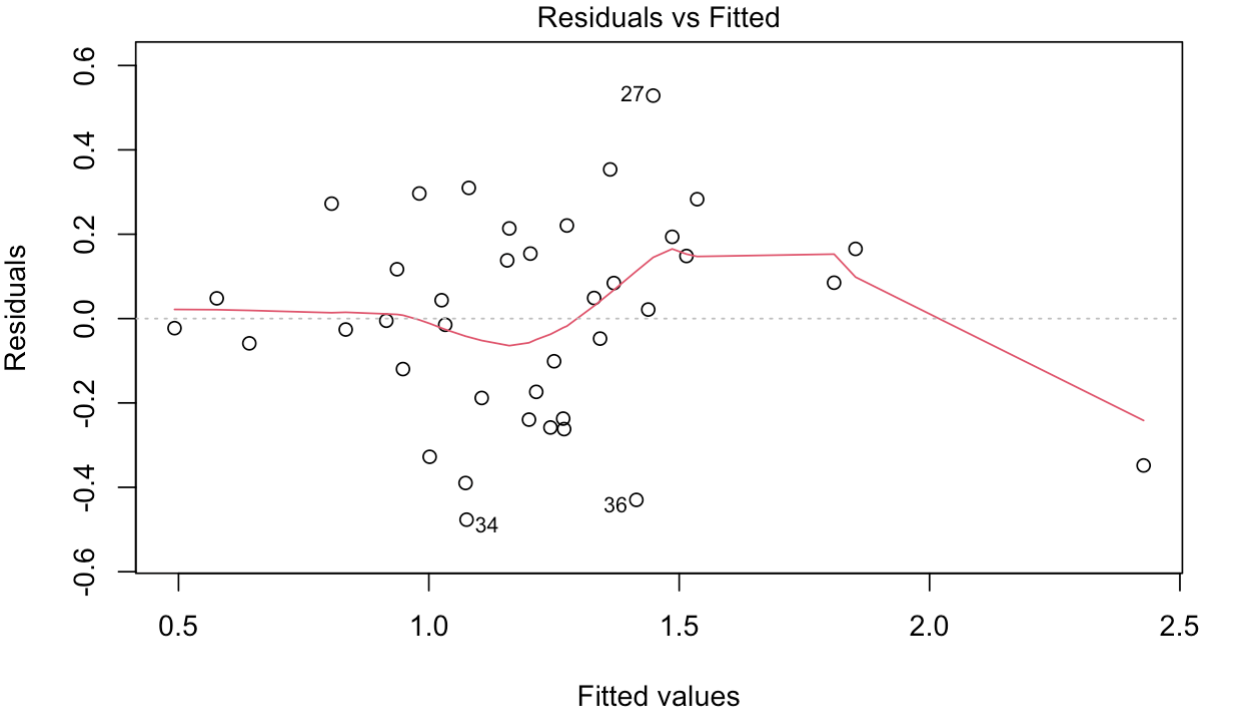
\includegraphics[width=1\textwidth]{Adequacy tests/BC plot.png}
    \caption{Plot of Residuals Against Fitted Values Post Box-Cox Transformation} \label{fig:AT3}
\end{figure}
\noindent

\begin{figure}[H]
    \centering
    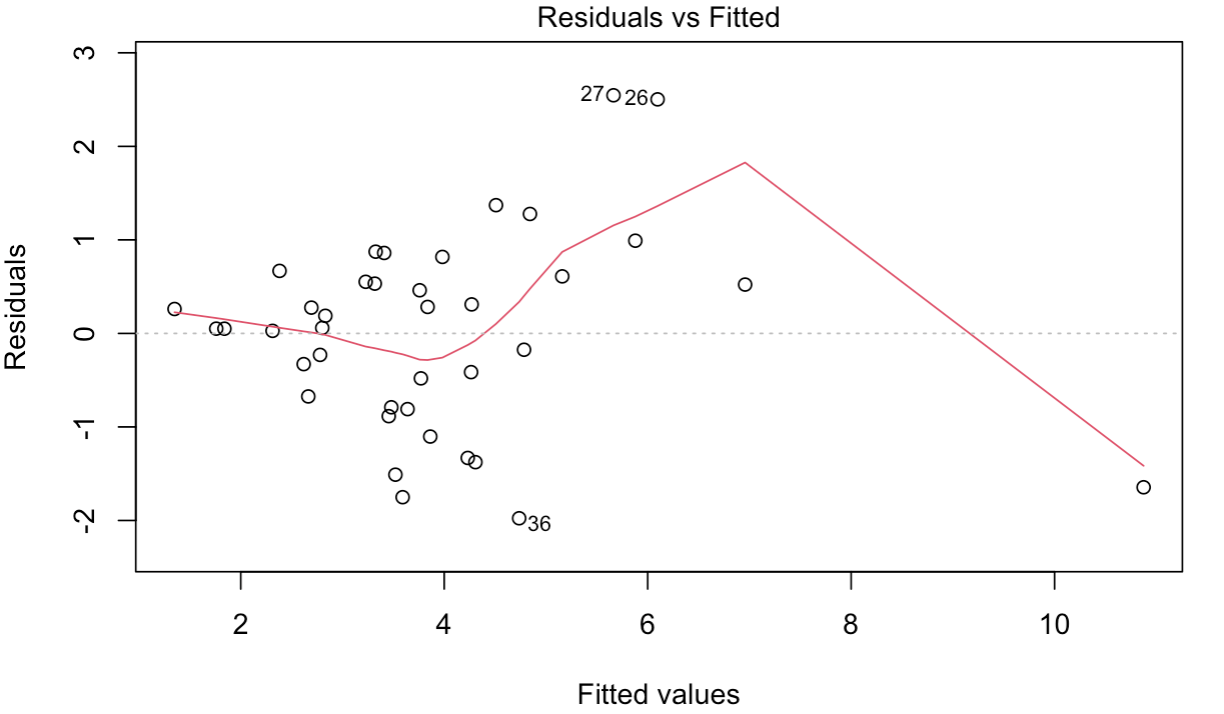
\includegraphics[width=1\textwidth]{Adequacy tests/WT plot.png}
    \caption{Plot of Residuals Against Fitted Values Weighted Least Squares Regression} \label{fig:AT4}
\end{figure}
\noindent

\begin{figure}[H]
    \centering
    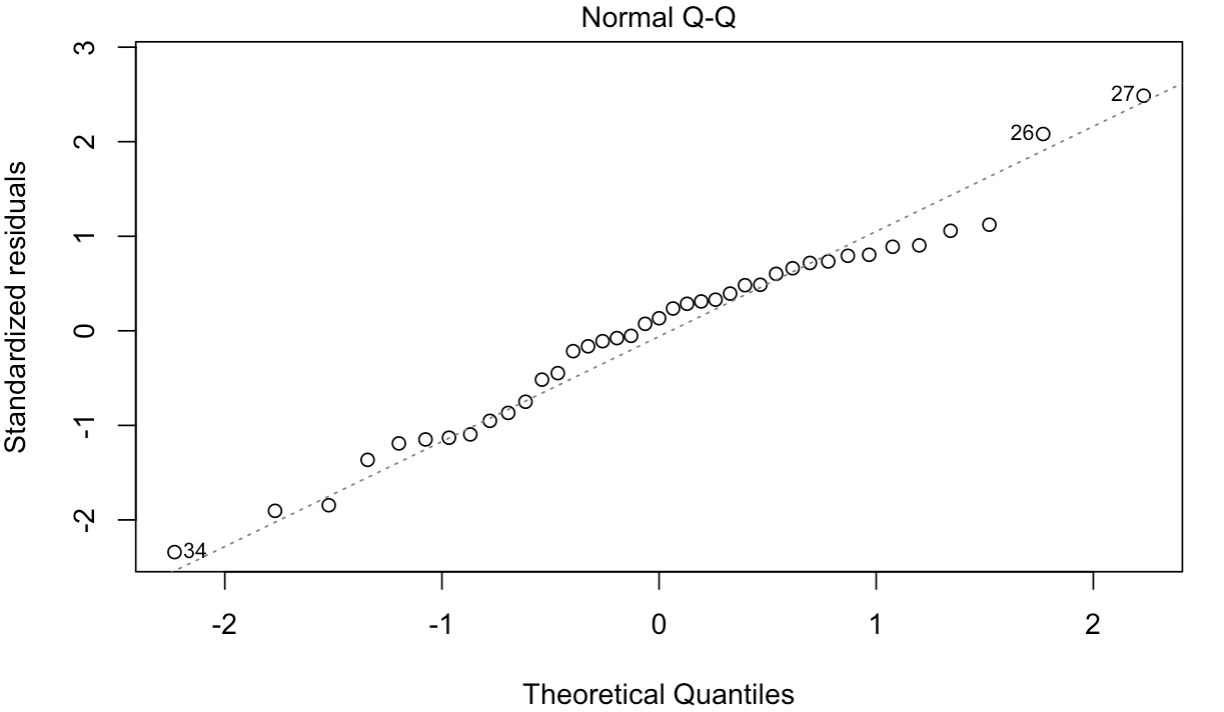
\includegraphics[width=1\textwidth]{Adequacy tests/QQ plot.png}
    \caption{Normal Quantile-Quantile Plot} \label{fig:AT5}
\end{figure}
\noindent

\begin{figure}[H]
    \centering
    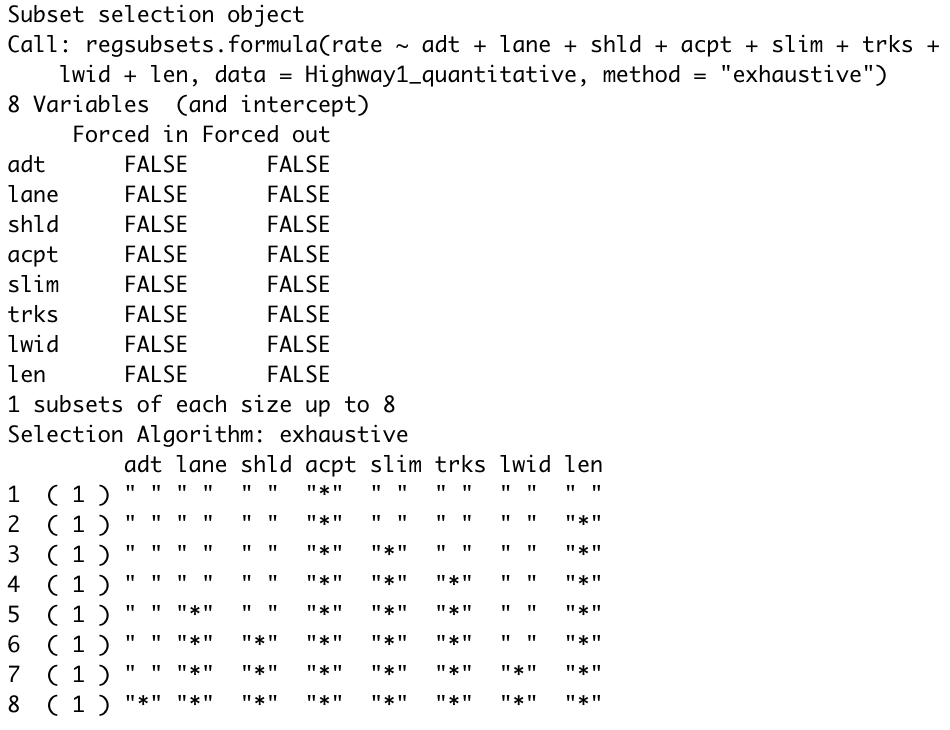
\includegraphics[width=0.65\textwidth]{Variable Selection/ST562 Subset Summary.png}
    \caption{Summary of Best Subset Models} \label{fig:VS1}
\end{figure}
\noindent

\begin{figure}[H]
    \centering
    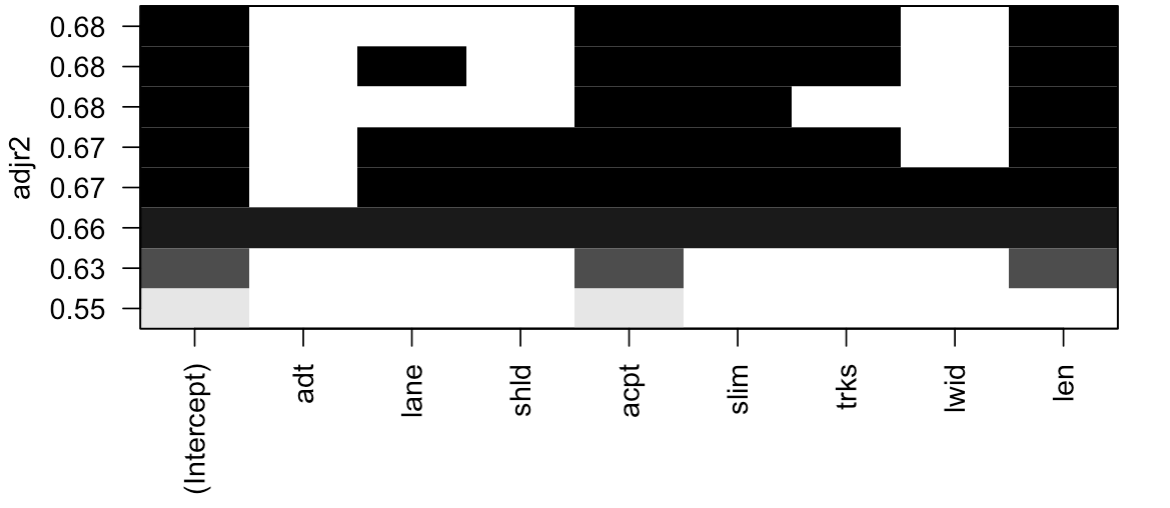
\includegraphics[width=0.9\textwidth]{Variable Selection/ST562 R^2.png}
    \caption{Best Subset of Predictors Using Adjusted $R^{2}$} \label{fig:VS2}
\end{figure}
\noindent

\begin{figure}[H]
    \centering
    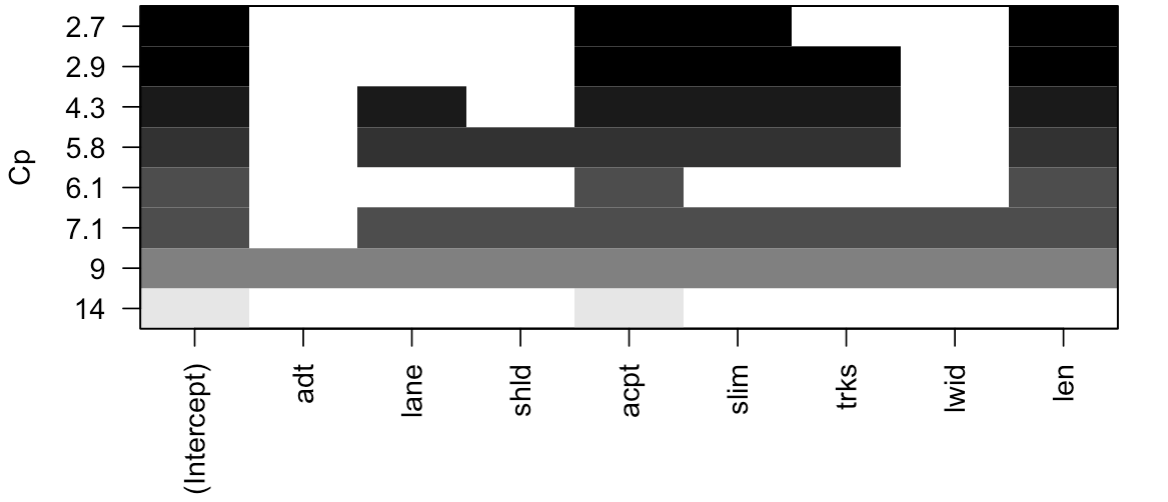
\includegraphics[width=0.9\textwidth]{Variable Selection/ST562 Cp.png}
    \caption{Best Subset of Predictors Using Mallow's $C_{p}$} \label{fig:VS3}
\end{figure}
\noindent

\section{R Code}
\subsection{Preliminary Remarks}
\begin{lstlisting}[language=R]
    rate<-Highway1$rate
    traffic<-Highway1$adt
    trucks<-Highway1$trks
    speed<-Highway1$slim
    lanes<-Highway1$lane
    width<-Highway1$lwid
    shoulder<-Highway1$shld
    access<-Highway1$acpt
    length<-Highway1$len

    plot(length,rate)
    plot(traffic,rate)
    plot(lanes,rate)
    plot(shoulder,rate)
    plot(access,rate)
    plot(speed,rate)
    plot(trucks,rate)
    plot(width,rate)
\end{lstlisting}

\subsection{Non-parametric Regression}
\begin{lstlisting}[language=R]
    y<-Highway1$rate
    x1<-Highway1$adt
    x2<-Highway1$trks
    x3<-Highway1$slim
    x4<-Highway1$lane
    x5<-Highway1$lwid
    x6<-Highway1$shld
    x7<-Highway1$acpt
    x8<-Highway1$len

    h1 <- dpill(x1, y)
    nonpara.fit1 <- locpoly(x1, y,degree=1,bandwidth=h1,gridsize=length(x1))
    mhat11<-nonpara.fit1$y
    x01<-nonpara.fit1$x
    plot(x1,y)
    lines(x01,mhat11,col="black")
    
    h2 <- dpill(x2, y)
    nonpara.fit1 <- locpoly(x2, y,degree=1,bandwidth=h2,gridsize=length(x2))
    mhat11<-nonpara.fit1$y
    x01<-nonpara.fit1$x
    plot(x2,y)
    lines(x01,mhat11,col="black")
    
    h3 <- dpill(x3, y)
    nonpara.fit1 <- locpoly(x3, y,degree=1,bandwidth=h3,gridsize=length(x3))
    mhat11<-nonpara.fit1$y
    x01<-nonpara.fit1$x
    plot(x3,y)
    lines(x01,mhat11,col="black")
    
    h4 <- dpill(x4, y)
    nonpara.fit1 <- locpoly(x4, y,degree=1,bandwidth=h4,gridsize=length(x4))
    mhat11<-nonpara.fit1$y
    x01<-nonpara.fit1$x
    plot(x4,y)
    lines(x01,mhat11,col="black")
    
    h5 <- dpill(x5, y)
    nonpara.fit1 <- locpoly(x5, y,degree=1,bandwidth=h5,gridsize=length(x5))
    mhat11<-nonpara.fit1$y
    x01<-nonpara.fit1$x
    plot(x5,y)
    lines(x01,mhat11,col="black")
    
    h6 <- dpill(x6, y)
    nonpara.fit1 <- locpoly(x6, y,degree=1,bandwidth=h6,gridsize=length(x6))
    mhat11<-nonpara.fit1$y
    x01<-nonpara.fit1$x
    plot(x6,y)
    lines(x01,mhat11,col="black")
    
    h7 <- dpill(x7, y)
    nonpara.fit1 <- locpoly(x7, y,degree=1,bandwidth=h7,gridsize=length(x7))
    mhat11<-nonpara.fit1$y
    x01<-nonpara.fit1$x
    plot(x7,y)
    lines(x01,mhat11,col="black")
    
    h8 <- dpill(x8, y)
    nonpara.fit1 <- locpoly(x8, y,degree=1,bandwidth=h8,gridsize=length(x8))
    mhat11<-nonpara.fit1$y
    x01<-nonpara.fit1$x
    plot(x8,y)
    lines(x01,mhat11,col="black")
\end{lstlisting}

\subsection{Diagnostic Check}
\begin{lstlisting}
    Highway_quantitative = Highway[,!(colnames(Highway) %in% c("name"))]
    corrgram(Highway_quantitative, order=TRUE, upper.panel=panel.cor)

    vif(fit_model_1)

    hat_values <- hatvalues(fit_model_1)
    threshold_lev <- (2*length(coef(fit_model_1))/length(hat_values))
    high_leverage<-hat_values[hat_values> threshold_lev]
    high_leverage

    stand_residuals <- rstandard(fit_model_1)
    outlier_observations<-stand_residuals[abs(stand_residuals) > 3]
    outlier_observations

    cooks_dist <- cooks.distance(fit_model_1)
    influential_observations<-cooks_dist[cooks_dist > 1]
    influential_observations
\end{lstlisting}

\subsection{Model Adequacy Testing}
\begin{lstlisting}
    plot(fit_model_1,1)
    plot(fit_model_1,2)
    plot(fit_model_1,3)

    bptest(fit_model_1)

    wt <- 1 / lm(abs(fit_model_1$residuals) ~ 
    fit_model_1$fitted.values)$fitted.values^2
    fit_model_4 <- lm(rate~adt+lane+shld+acpt+slim+trks+lwid+len,
    data = Highway1, weights=wt)
    
    boxcox <- boxcox(fit_model_1)
    lambda<-boxcox$x[which.max(boxcox$y)]
    lambda
    fit_model_5 <- lm(((rate^lambda - 1)/lambda)~adt+lane+shld+acpt+slim
    +trks+lwid+len, data = Highway1)

    summary(fit_model_1)
    summary(fit_model_4)
    summary(fit_model_5)

    plot(fit_model_1,1)
    plot(fit_model_4,1)
    plot(fit_model_5,1)

    bptest(fit_model_4)
    bptest(fit_model_5)

    dwtest(fit_model_1)
\end{lstlisting}

\subsection{Variable Selection}
\begin{lstlisting}
    Highway1_quantitative <- Highway1[,!(colnames(Highway1) 
    %in% c( "name"))]

    reg_example <-  regsubsets(rate~adt+lane+shld+acpt+slim+trks+lwid
    +len,data = Highway1_quantitative,  method = "exhaustive")
    reg_summary_example <- summary(reg_example)
    reg_summary_example

    names(reg_summary_example) 
    reg_summary_example$cp
    data.frame(
      Adj.R2 = which.max(reg_summary_example$adjr2),
      CP = which.min(reg_summary_example$cp))
    plot_adjr2 <- plot(reg_example, scale = "adjr2")
    plot_adjr2
    plot_cp <- plot(reg_example, scale = "Cp")
    plot_cp
\end{lstlisting}

\subsection{Hypothesis Tests}
\begin{lstlisting}
    fit_model_1<-lm(rate~adt+lane+shld+acpt+slim+trks+lwid+len,
    data = Highway1)
    summary(fit_model_1)

    fit.model.null<-lm(rate~1, data = Highway1)
    anova(fit.model.null,fit_model_1)

    fit_model_7 <- lm(rate~acpt+slim+trks+len, data = Highway1)
    plot(fit_model_7,1)
    summary(fit_model_7)

    fit.model.null<-lm(rate~1, data = Highway1)
    anova(fit.model.null,fit_model_7)
\end{lstlisting}
\end{document}
